% =====================================================================
%  מבוא לקוסמולוגיה — רשימות הרצאה (9 שעות, 3 מפגשים × 3 שעות)
%  קומפילציה: lualatex cosmo_lectures.tex  (פעמיים)
%  פתרונות התרגילים: solutions.tex (למרצה)
% =====================================================================
\documentclass[11pt,a4paper]{article}
% =====================================================================
%  Shared preamble — lecture notes "Introduction to Cosmology" (9 h)
%  Compile:  lualatex cosmo_lectures.tex   (twice, for the TOC)
% =====================================================================
\usepackage[a4paper,top=2.2cm,bottom=2.2cm,left=2.2cm,right=2.2cm]{geometry}
\usepackage{fontspec}
\usepackage{amsmath,amssymb}
\usepackage[bidi=basic]{babel}
\babelprovide[import,main]{hebrew}
\babelprovide[import]{english}

% ---- fonts: Culmus (Overleaf/Linux) -> Windows David -> FreeSerif ----
\IfFontExistsTF{David CLM}{%
  \babelfont{rm}{David CLM}\babelfont{sf}{Simple CLM}\babelfont{tt}{Miriam Mono CLM}%
}{\IfFontExistsTF{David}{%
  \babelfont{rm}[ItalicFeatures={FakeSlant=0.15}]{David}\babelfont{sf}{Arial}\babelfont{tt}{Courier New}%
}{\IfFileExists{/mnt/c/Windows/Fonts/david.ttf}{%
  \babelfont{rm}[Path=/mnt/c/Windows/Fonts/,Extension=.ttf,BoldFont=davidbd,ItalicFont=david,
    ItalicFeatures={FakeSlant=0.15}]{david}%
  \babelfont{sf}[Path=/mnt/c/Windows/Fonts/,Extension=.ttf,BoldFont=arialbd]{arial}%
  \babelfont{tt}[Path=/mnt/c/Windows/Fonts/,Extension=.ttf]{cour}%
}{%
  \babelfont{rm}{FreeSerif}\babelfont{sf}{FreeSans}\babelfont{tt}{FreeMono}%
}}}
\babelfont[english]{rm}{Latin Modern Roman}
\babelfont[english]{tt}{Latin Modern Mono}

\usepackage{xcolor}
\usepackage[framemethod=default]{mdframed}
\usepackage{enumitem}
\usepackage{booktabs}
\usepackage{graphicx}
\usepackage{fancyhdr}
\usepackage{needspace}
\usepackage{listings}
\usepackage[hidelinks]{hyperref}
\lstset{basicstyle=\ttfamily\footnotesize,keywordstyle=\color{qblue}\bfseries,
  commentstyle=\color{ggreen}\itshape,frame=single,rulecolor=\color{black!30},
  backgroundcolor=\color{black!2},breaklines=true,showstringspaces=false,
  language=Python,columns=fullflexible}

\renewcommand{\labelitemi}{\ensuremath{\bullet}}
\renewcommand{\labelitemii}{\ensuremath{\circ}}
\setlist[itemize]{leftmargin=1.4em,itemsep=1pt,topsep=2pt}
\setlist[enumerate]{leftmargin=1.6em,itemsep=1pt,topsep=2pt}

% ---- colours (as in the original course) ----
\definecolor{qblue}{RGB}{20,60,120}
\definecolor{ggreen}{RGB}{20,100,70}
\definecolor{kpurple}{RGB}{95,45,110}
\definecolor{worange}{RGB}{170,90,10}

\newmdenv[linecolor=kpurple,linewidth=1pt,backgroundcolor=kpurple!4,
  innertopmargin=6pt,innerbottommargin=6pt,innerleftmargin=8pt,innerrightmargin=8pt,
  skipabove=7pt,skipbelow=7pt]{keybox}
\newmdenv[linecolor=worange,linewidth=1pt,backgroundcolor=worange!5,
  innertopmargin=6pt,innerbottommargin=6pt,innerleftmargin=8pt,innerrightmargin=8pt,
  skipabove=7pt,skipbelow=7pt]{warnbox}
\newmdenv[linecolor=ggreen,linewidth=1pt,backgroundcolor=ggreen!5,
  innertopmargin=6pt,innerbottommargin=6pt,innerleftmargin=8pt,innerrightmargin=8pt,
  skipabove=7pt,skipbelow=7pt]{goalbox}
\newmdenv[linecolor=qblue,linewidth=1.1pt,backgroundcolor=qblue!5,
  innertopmargin=6pt,innerbottommargin=6pt,innerleftmargin=8pt,innerrightmargin=8pt,
  skipabove=8pt,skipbelow=6pt]{exbox}
\newmdenv[linecolor=black!35,linewidth=0.7pt,backgroundcolor=black!3,
  innertopmargin=6pt,innerbottommargin=6pt,innerleftmargin=8pt,innerrightmargin=8pt,
  skipabove=4pt,skipbelow=8pt]{solbox}

% ---- macros ----
\newcommand{\en}[1]{\foreignlanguage{english}{#1}}
\newcommand{\Msun}{M_{\odot}}
\newcommand{\Mpc}{\mathrm{Mpc}}
\newcommand{\kpc}{\mathrm{kpc}}
\newcommand{\Gyr}{\mathrm{Gyr}}
\newcommand{\kms}{\mathrm{km\,s^{-1}}}
\newcommand{\kmsMpc}{\mathrm{km\,s^{-1}\,Mpc^{-1}}}
\newcommand{\LCDM}{\Lambda\mathrm{CDM}}

% lecture header: \lecture{number}{title}{time budget + one-line content}
\newcounter{lec}
\counterwithin*{subsection}{lec}
\renewcommand{\thesubsection}{\thelec.\arabic{subsection}}
\makeatletter\renewcommand{\fps@figure}{htbp}\makeatother
\newcommand{\lecture}[3]{%
  \clearpage\refstepcounter{lec}%
  \noindent\colorbox{qblue}{\parbox{\dimexpr\textwidth-2\fboxsep}{%
   \color{white}\bfseries\Large הרצאה #1: #2\\[3pt]\normalsize\mdseries #3}}%
  \addcontentsline{toc}{section}{הרצאה #1: #2}\par\medskip}

% exercises: numbered per lecture (1.1, 1.2, ...)
\newcounter{ex}[lec]
\newenvironment{exercise}[1]{%
  \refstepcounter{ex}\begin{exbox}\textbf{\textcolor{qblue}{תרגיל \thelec.\theex\ --- #1.}}\ }%
  {\end{exbox}}
\newcommand{\soln}[1]{\par\smallskip\noindent\textbf{פתרון #1.}\ }

\pagestyle{fancy}\fancyhf{}
\fancyhead[R]{\small מבוא לקוסמולוגיה --- רשימות הרצאה}
\fancyhead[L]{\small\hbox{\textdir TLT\relax\thepage}}
\renewcommand{\headrulewidth}{0.4pt}
\setlength{\parindent}{0pt}\setlength{\parskip}{4pt}


\begin{document}

\begin{center}
{\LARGE\bfseries מבוא לקוסמולוגיה}\\[6pt]
{\large רשימות הרצאה --- 9 שעות (שלושה מפגשים בני שלוש שעות)}\\[4pt]
{\normalsize שנה ג' בפיזיקה / תואר שני, שלב מתחילים}
\end{center}

\subsection*{מפת הקורס}
\begin{center}\small
\begin{tabular}{@{}clll@{}}
\toprule
מפגש & זמן & הרצאה & מה לוקחים הביתה \\ \midrule
1 & 2 ש' & 1. משוואות פרידמן, פתרונות, זמנים ומרחקים & $H(z)$, $t_0$, $D_M,D_A,D_L$ \\
  & 1 ש' & 2א. הסקה בייסיאנית ו-\en{MCMC} & נראות, מוקדמת, דגימה, אבחון \\ \midrule
2 & 1 ש' & 2ב. סופרנובות ואנרגיה אפלה (מחברת \en{Pantheon+}) & $\mu(z)$, ההיסט $\mathcal M$, $(\Omega_m,w)$ \\
  & 1 ש' & 3. חומר אפל והרשת הקוסמית: הפרעות ואורך ג'ינס & $\ddot\delta+2H\dot\delta=4\pi G\bar\rho\delta$, $\lambda_J$ \\
  & 1 ש' & 4. עדויות לחומר אפל: ויריאל, קריסה כדורית, עקומות סיבוב, \en{NFW}, \en{MOND} & $M=5\sigma^2R/G$, $\delta_c$, $18\pi^2$, $v_c(r)$ \\ \midrule
3 & 1.5 ש' & 5. היקום החם, הסקאלה האקוסטית ו-\en{BAO} (\en{DESI}) & $r_s$, $\theta_\star$, $D/r_d$, המתחים \\
  & 1.5 ש' & 6. אינפלציה & $\epsilon,\eta$, $n_s$, $r$ \\ \bottomrule
\end{tabular}
\end{center}

בכל הרצאה: מטרות, תיאוריה בקיצור, ובסופה 3 תרגילים שנפתרים בכיתה אחרי התיאוריה; הפתרון המלא מופיע בתיבה אפורה מיד אחרי כל תרגיל.

\textbf{מוסכמות.} $c=1$ רק כשנאמר במפורש. $a_0=1$, $1+z=1/a$, $H_0=100\,h\,\kmsMpc$, $c/H_0=2998\,h^{-1}\Mpc$, $1/H_0=9.78\,h^{-1}\Gyr$. ערכי ייחוס (\en{Planck 2018}): $h=0.674$, $\Omega_m=0.315$, $\Omega_bh^2=0.0224$, $\Omega_mh^2=0.143$.

\tableofcontents

% =====================================================================
\lecture{1}{משוואות פרידמן, פתרונות, זמנים ומרחקים}{מפגש 1, שעתיים. \ (15' ניוטון, 25' גזירה מ-\en{GR}, 30' פתרונות, 50' זמנים ומרחקים + תרגילים)}
% =====================================================================

\begin{goalbox}
\textbf{מטרות.} (1) לגזור את משוואות פרידמן (ניוטונית, ואז לראות מה \en{GR} מוסיפה). (2) לפתור אותן לרכיב בודד ולחומר${}+\Lambda$. (3) לחשב גיל, זמן מבט-לאחור ושלושת המרחקים $D_M$, $D_A$, $D_L$.
\end{goalbox}

\subsection{התפשטות, מקדם הקנה מידה, הסחה לאדום}
העקרון הקוסמולוגי (הומוגניות ואיזוטרופיות) משאיר דרגת חופש אחת: $a(t)$. מרחק פיזיקלי בין שני גופים נעים: $r=a(t)\,x$, עם $x$ קבוע. גזירה:
\begin{equation}
\dot r=\frac{\dot a}{a}\,r\equiv H(t)\,r \qquad(\text{חוק האבל}).
\end{equation}
אורך הגל נמתח יחד עם המרחב, $\lambda\propto a$, ולכן
\begin{equation}
1+z=\frac{\lambda_{\rm obs}}{\lambda_{\rm em}}=\frac{1}{a(t_{\rm em})} .
\end{equation}
המטריקה (\en{FLRW}), עם $k=0,\pm1$ ו-$S_k(\chi)=\sin\chi,\ \chi,\ \sinh\chi$:
\begin{equation}
ds^2=-c^2dt^2+a^2(t)\left[d\chi^2+S_k^2(\chi)\,d\Omega^2\right].
\end{equation}

\subsection{משוואות פרידמן}
\textbf{גזירה ניוטונית.} כדור ברדיוס $r=ax$ וצפיפות $\rho$. אנרגיה של חלקיק בשפה:
\begin{equation}
\frac12\dot r^2-\frac{GM}{r}=E,\qquad M=\frac{4\pi}{3}\rho r^3
\quad\Longrightarrow\quad
H^2=\frac{8\pi G}{3}\rho-\frac{kc^2}{a^2},
\end{equation}
כאשר $kc^2\equiv-2E/x^2$ קבוע. \emph{האנרגיה הכוללת היא העקמומיות.}

\textbf{הגבול של הגזירה הניוטונית.} היא נותנת את המשוואה הראשונה, אבל לא אומרת מה עושה הלחץ, ומניחה מרחב אוקלידי ואינסופי עם מרכז שרירותי. ב-\en{GR} אין את הבעיות האלה.

\subsection{גזירה מיחסות כללית}
\emph{עובדים ב-$c=1$; בסוף מחזירים $c$. ראשית נגזור את המקרה השטוח ($k=0$) עד הסוף, ואז נוסיף עקמומיות ו-$\Lambda$.}

\textbf{שלב 0: מה צריך.} משוואות איינשטיין, $G_{\mu\nu}\equiv R_{\mu\nu}-\tfrac12g_{\mu\nu}R=8\pi G\,T_{\mu\nu}$, עם
\begin{equation}
\Gamma^\lambda_{\mu\nu}=\tfrac12g^{\lambda\sigma}\big(\partial_\mu g_{\sigma\nu}+\partial_\nu g_{\sigma\mu}-\partial_\sigma g_{\mu\nu}\big),\qquad
R_{\mu\nu}=\partial_\lambda\Gamma^\lambda_{\mu\nu}-\partial_\nu\Gamma^\lambda_{\mu\lambda}+\Gamma^\lambda_{\lambda\sigma}\Gamma^\sigma_{\mu\nu}-\Gamma^\lambda_{\nu\sigma}\Gamma^\sigma_{\mu\lambda}.
\label{eq:ricci-def}
\end{equation}

\textbf{שלב 1: המטריקה.} בקואורדינטות נעות קרטזיות, $ds^2=-dt^2+a^2(t)\,\delta_{ij}dx^idx^j$, כלומר
\begin{equation}
g_{00}=-1,\quad g_{ij}=a^2\delta_{ij},\quad g^{00}=-1,\quad g^{ij}=a^{-2}\delta^{ij}.
\end{equation}
הרכיב היחיד שתלוי במשהו הוא $g_{ij}$, והוא תלוי רק ב-$t$. לכן רק נגזרות $\partial_0g_{ij}=2a\dot a\,\delta_{ij}$ שורדות.

\textbf{שלב 2: סמלי כריסטופל.} מציבים ב-\eqref{eq:ricci-def}. רק שני סוגים אינם אפס:
\begin{equation}
\boxed{\;\Gamma^0_{ij}=a\dot a\,\delta_{ij},\qquad \Gamma^i_{0j}=\Gamma^i_{j0}=\frac{\dot a}{a}\,\delta^i_j=H\delta^i_j\;}
\end{equation}
לדוגמה: $\Gamma^0_{ij}=\tfrac12g^{00}(-\partial_0g_{ij})=\tfrac12\cdot2a\dot a\,\delta_{ij}$. כל השאר ($\Gamma^0_{00}$, $\Gamma^0_{0i}$, $\Gamma^i_{00}$, $\Gamma^i_{jk}$) מתאפסים, כי $g_{00}$ קבוע ו-$g_{ij}$ לא תלוי ב-$x$. \emph{פירוש:} $\Gamma^i_{0j}$ הוא "חיכוך האבל" במשוואת הגאודזה, $\dot p\propto-Hp$, כלומר $p\propto1/a$; לכן אורכי גל נמתחים.

\textbf{שלב 3: טנזור ריצ'י.} הרכיב $00$, איבר אחר איבר ב-\eqref{eq:ricci-def}:
\begin{equation}
R_{00}=\underbrace{\partial_\lambda\Gamma^\lambda_{00}}_{0}-\underbrace{\partial_0\Gamma^\lambda_{0\lambda}}_{\partial_0(3\dot a/a)}+\underbrace{\Gamma^\lambda_{\lambda\sigma}\Gamma^\sigma_{00}}_{0}-\underbrace{\Gamma^\lambda_{0\sigma}\Gamma^\sigma_{0\lambda}}_{\Gamma^i_{0j}\Gamma^j_{0i}=3H^2}
=-3\Big(\frac{\ddot a}{a}-\frac{\dot a^2}{a^2}\Big)-3\frac{\dot a^2}{a^2}
=-3\frac{\ddot a}{a}.
\end{equation}
הרכיבים $ij$:
\begin{equation}
R_{ij}=\underbrace{\partial_0\Gamma^0_{ij}}_{(\dot a^2+a\ddot a)\delta_{ij}}-\underbrace{\partial_j\Gamma^\lambda_{i\lambda}}_{0}+\underbrace{\Gamma^\lambda_{\lambda0}\Gamma^0_{ij}}_{3H\cdot a\dot a\,\delta_{ij}}-\underbrace{\big(\Gamma^0_{jk}\Gamma^k_{i0}+\Gamma^k_{j0}\Gamma^0_{ik}\big)}_{2\dot a^2\delta_{ij}}
=\big(a\ddot a+2\dot a^2\big)\delta_{ij}.
\end{equation}
$R_{0i}=0$ מאיזוטרופיות: אין כיוון מועדף שאליו וקטור יכול להצביע.

\textbf{שלב 4: סקלר ריצ'י וטנזור איינשטיין.}
\begin{equation}
R=g^{00}R_{00}+g^{ij}R_{ij}=3\frac{\ddot a}{a}+\frac{3(a\ddot a+2\dot a^2)}{a^2}=6\Big(\frac{\ddot a}{a}+\frac{\dot a^2}{a^2}\Big),
\end{equation}
\begin{equation}
\boxed{\;G_{00}=R_{00}+\tfrac12R=3\frac{\dot a^2}{a^2},\qquad
G_{ij}=R_{ij}-\tfrac12a^2\delta_{ij}R=-\big(2a\ddot a+\dot a^2\big)\delta_{ij}\;}
\end{equation}
שימו לב: ב-$G_{00}$ \emph{אין} $\ddot a$. זו משוואת אילוץ (כמו חוק גאוס באלקטרומגנטיות), לא משוואת תנועה.

\textbf{שלב 5: המקור.} נוזל מושלם במנוחה בקואורדינטות הנעות, $u^\mu=(1,0,0,0)$, $u_\mu=(-1,0,0,0)$:
\begin{equation}
T_{\mu\nu}=(\rho+p)u_\mu u_\nu+p\,g_{\mu\nu}\quad\Longrightarrow\quad T_{00}=\rho,\qquad T_{ij}=p\,a^2\delta_{ij}.
\end{equation}
זו הצורה היחידה שמתאימה לסימטריה: הומוגניות דורשת $\rho(t)$, $p(t)$, ואיזוטרופיות דורשת $T_{0i}=0$ ו-$T_{ij}\propto\delta_{ij}$.

\textbf{שלב 6: שתי המשוואות.}
\begin{align}
00:\qquad &3\frac{\dot a^2}{a^2}=8\pi G\rho &&\Longrightarrow\quad H^2=\frac{8\pi G}{3}\rho ,\\
ij:\qquad &-\big(2a\ddot a+\dot a^2\big)=8\pi G\,p\,a^2 &&\Longrightarrow\quad 2\frac{\ddot a}{a}+H^2=-8\pi Gp .
\end{align}
מציבים את $H^2$ מהראשונה בשנייה: $2\ddot a/a=-8\pi G(p+\rho/3)$, כלומר
\begin{equation}
\frac{\ddot a}{a}=-\frac{4\pi G}{3}\big(\rho+3p\big).
\end{equation}

\textbf{שלב 7: שימור, בחינם.} זהות ביאנקי $\nabla^\mu G_{\mu\nu}\equiv0$ מחייבת $\nabla^\mu T_{\mu\nu}=0$. הרכיב $\nu=0$:
\begin{equation}
\nabla_\mu T^{\mu0}=\partial_0T^{00}+\Gamma^\mu_{\mu0}T^{00}+\Gamma^0_{ij}T^{ij}
=\dot\rho+3H\rho+a\dot a\,\delta_{ij}\,\frac{p}{a^2}\delta^{ij}
=\dot\rho+3H(\rho+p)=0 .
\end{equation}
אותה תוצאה מתקבלת אם גוזרים את משוואת $00$ בזמן ומציבים את משוואת $ij$. לכן רק \emph{שתיים} משלוש המשוואות בלתי תלויות. בפועל עובדים עם פרידמן הראשונה ומשוואת השימור.

\textbf{שלב 8: עקמומיות ו-$\Lambda$.}
\begin{itemize}
\item \textbf{$k\neq0$.} עם $g_{ij}=a^2\gamma_{ij}$, כאשר $\gamma_{ij}$ מטריקה של מרחב בעל עקמומיות קבועה, למרחב הזה יש ריצ'י משלו: ${}^{(3)}\!R_{ij}=2k\gamma_{ij}$. התוצאה: $G_{00}=3\big(H^2+k/a^2\big)$ ו-$G_{ij}=-\big(2a\ddot a+\dot a^2+k\big)\gamma_{ij}$. המשוואה הראשונה מקבלת $-k/a^2$; משוואת התאוצה לא משתנה ($k$ מתבטל בהפרש).
\item \textbf{$\Lambda$.} $G_{\mu\nu}+\Lambda g_{\mu\nu}=8\pi GT_{\mu\nu}$. העברה לאגף ימין מראה ש-$\Lambda$ הוא נוזל עם $\rho_\Lambda=\Lambda/8\pi G$ ו-$p_\Lambda=-\rho_\Lambda$. שימו לב ש-$\rho_\Lambda+3p_\Lambda=-2\rho_\Lambda<0$: כבידה דוחה.
\end{itemize}
מחזירים $c$ ($\rho\to\rho c^2$ בצפיפות אנרגיה, $k\to kc^2$, $\Lambda\to\Lambda c^2$) ומקבלים:
\begin{equation}
\boxed{\;H^2=\frac{8\pi G}{3}\rho-\frac{kc^2}{a^2}+\frac{\Lambda c^2}{3},\qquad
\frac{\ddot a}{a}=-\frac{4\pi G}{3}\Big(\rho+\frac{3p}{c^2}\Big)+\frac{\Lambda c^2}{3}\;}
\label{eq:friedmann}
\end{equation}

\begin{keybox}
\textbf{תסריט ללוח (כ-25 דקות).} מטריקה $\to$ שני סוגי $\Gamma$ $\to$ $R_{00}$ ו-$R_{ij}$ (לעשות לפחות את $R_{00}$ איבר אחר איבר) $\to$ $R$ $\to$ $G_{00}$, $G_{ij}$ $\to$ $T_{\mu\nu}$ $\to$ שתי משוואות $\to$ ביאנקי נותן שימור. \emph{נקודות לעצור עליהן:} (1) $G_{00}$ בלי $\ddot a$ = אילוץ; (2) $\rho+3p$ במשוואת התאוצה; (3) $k$ נכנס דרך העקמומיות של המרחב התלת-ממדי, לא דרך $a$.
\end{keybox}

ההבדל המהותי: \textbf{הלחץ כובד}. זה מה שניוטון לא יכול לתת, ובזכותו $p<-\rho c^2/3$ מאיץ.
משוואת השימור (שלב 7; או בתרמודינמיקה, $dE=-p\,dV$) נותנת את התלות של כל רכיב ב-$a$:
\begin{equation}
\dot\rho+3H\Big(\rho+\frac{p}{c^2}\Big)=0
\quad\xrightarrow{\;p=w\rho c^2\;}\quad
\rho\propto a^{-3(1+w)}:\qquad
\begin{cases}
\text{חומר } (w=0): & \rho\propto a^{-3}\\
\text{קרינה } (w=\tfrac13): & \rho\propto a^{-4}\\
\Lambda\ (w=-1): & \rho=\text{const}
\end{cases}
\end{equation}

\textbf{פרמטרי צפיפות.} $\rho_c=3H^2/8\pi G$, $\Omega_i=\rho_i/\rho_c$, $\Omega_k=-kc^2/(a_0H_0)^2$. היום $\sum_i\Omega_{i}+\Omega_k=1$, ומשוואת פרידמן הופכת ל:
\begin{equation}
\boxed{\;E^2(z)\equiv\frac{H^2}{H_0^2}=\Omega_r(1+z)^4+\Omega_m(1+z)^3+\Omega_k(1+z)^2+\Omega_\Lambda\;}
\label{eq:Ez}
\end{equation}
ופרמטר התאוטה $q\equiv-\ddot a a/\dot a^2$ נותן היום $q_0=\tfrac12\Omega_m+\Omega_r-\Omega_\Lambda$.

\subsection{פתרונות}
\begin{keybox}
\textbf{רכיב בודד, $k=0$.} $\dot a^2\propto a^{-(1+3w)}$ נותן
\begin{equation}
a\propto t^{2/[3(1+w)]}:\qquad a\propto t^{1/2}\ (\text{קרינה}),\quad a\propto t^{2/3}\ (\text{חומר, \en{EdS}}),\quad a\propto e^{H_\Lambda t}\ (\Lambda).
\end{equation}
ב-\en{EdS}: $H=2/(3t)$, ולכן $t_0=\frac23H_0^{-1}=9.3\,\Gyr$ עבור $h=0.7$ --- צעיר מהכוכבים הזקנים ביותר ($\gtrsim12\,\Gyr$). זו הייתה רמז מוקדם ל-$\Lambda$.
\end{keybox}

\textbf{חומר${}+\Lambda$ ($k=0$), פתרון סגור.} עם $x=a^{3/2}$ המשוואה הופכת למשוואה לינארית ופתרונה
\begin{equation}
a(t)=\Big(\frac{\Omega_m}{\Omega_\Lambda}\Big)^{1/3}\sinh^{2/3}\!\Big(\tfrac32\sqrt{\Omega_\Lambda}\,H_0t\Big),
\qquad
t_0=\frac{2}{3H_0\sqrt{\Omega_\Lambda}}\,\mathrm{arsinh}\sqrt{\frac{\Omega_\Lambda}{\Omega_m}} .
\end{equation}
\textbf{מעברים.} $\rho_r=\rho_m$ ב-$1+z_{\rm eq}=\Omega_m/\Omega_r\approx3400$; $\rho_m=\rho_\Lambda$ ב-$z\approx0.33$; התאוצה מתחילה ($\ddot a=0$) ב-$1+z_{\rm acc}=(2\Omega_\Lambda/\Omega_m)^{1/3}$, כלומר $z_{\rm acc}\approx0.67$.

\textbf{עקמומיות.} ביקום של חומר בלבד: $k=+1$ קורס, $k=-1$ מתפשט לנצח ($a\propto t$ בגבול), $k=0$ על הגבול. עם $\Lambda$ הגורל נקבע על ידי $\Lambda$, לא על ידי $k$. העקמומיות דועכת לאט יותר מחומר וקרינה ($a^{-2}$), ולכן היא שולטת בעתיד אם $\Lambda=0$; זו "בעיית השטיחות" של הרצאה 6.

\begin{figure}[htbp]\centering
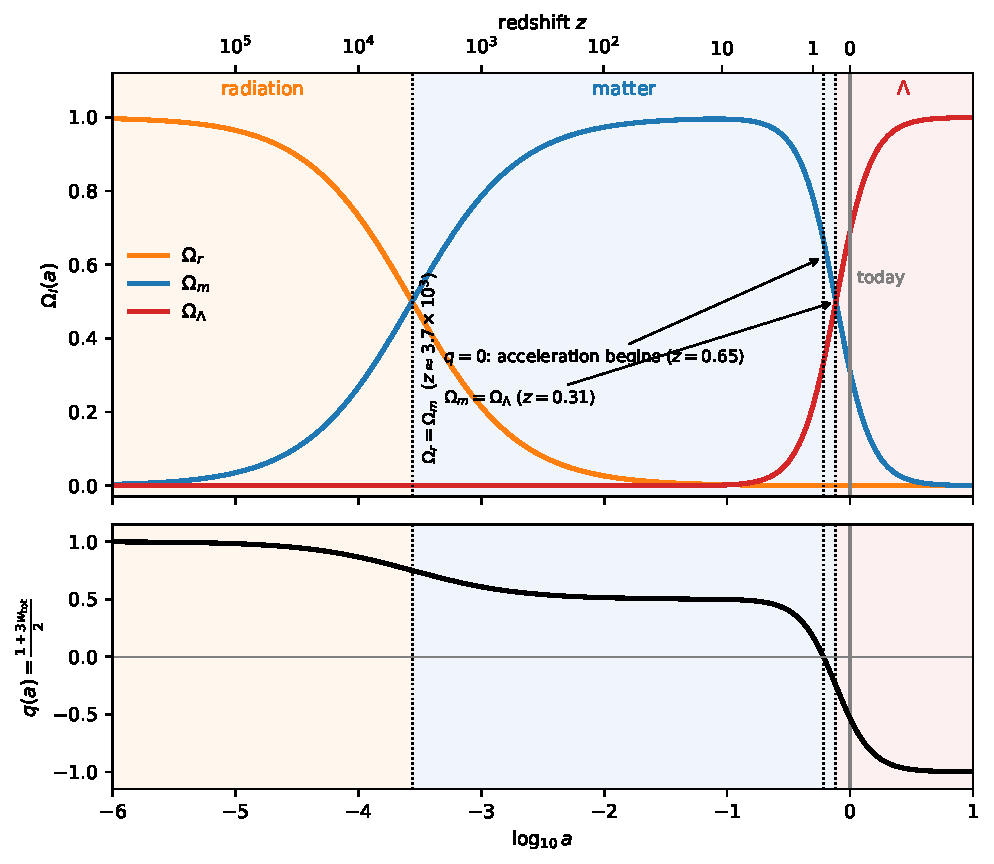
\includegraphics[width=0.75\textwidth]{figs/fig_omega_z.pdf}
\caption{\small $\Omega_i(z)$: עידן קרינה, עידן חומר ועידן $\Lambda$. המעברים ב-$z_{\rm eq}\approx3400$ וב-$z\approx0.3$.}
\end{figure}

\subsection{זמנים}
מ-$dt=da/(aH)$:
\begin{equation}
t(z)=\int_z^\infty\frac{dz'}{(1+z')H(z')},\qquad
t_{\rm lb}(z)=\int_0^z\frac{dz'}{(1+z')H(z')} .
\end{equation}
עבור $\Omega_m=0.3$, $h=0.7$: $t_0=13.5\,\Gyr$, ואור מ-$z=1$ יצא לפני $7.7\,\Gyr$. עם ערכי \en{Planck}: $t_0=13.8\,\Gyr$.

\textbf{אופק החלקיק} --- המרחק הנע הגדול ביותר שאור עבר מאז $t=0$: $\chi_{\rm p}=\int_0^{t}c\,dt'/a=\int_z^\infty c\,dz'/H$. ב-\en{EdS} $\chi_{\rm p}=2c/(a H)$, כלומר סופי. בגלל זה יש "בעיית אופק" (הרצאה 6).

\subsection{מרחקים}
כל המרחקים נבנים מהמרחק הנע לאורך קו הראייה (אור נע על $ds=0$, $c\,dt=a\,d\chi$):
\begin{keybox}
\begin{align}
D_C(z)&=\frac{c}{H_0}\int_0^z\frac{dz'}{E(z')},\\
D_M&=\frac{c}{H_0\sqrt{|\Omega_k|}}\,S_k\!\Big(\sqrt{|\Omega_k|}\,\frac{H_0D_C}{c}\Big)\ \ (=D_C\ \text{אם}\ k=0),\\
D_A&=\frac{D_M}{1+z}\quad(\text{גודל זוויתי: } \theta=\ell/D_A),\qquad
D_L=(1+z)\,D_M\quad(\text{שטף: } F=L/4\pi D_L^2).
\end{align}
יחס הדואליות $D_L=(1+z)^2D_A$ נכון בכל מטריקה שבה פוטונים נשמרים. שני גורמי $(1+z)$ ב-$D_L$: האנרגיה של כל פוטון יורדת, וקצב ההגעה שלהם יורד.
\end{keybox}
\textbf{גבול $z\ll1$:} $D\simeq cz/H_0\,[1+\tfrac12(1-q_0)z]$ ($D_L$). כלומר בסדר ראשון מודדים $H_0$, ובסדר שני את $q_0$, את התאוצה.

\textbf{תכונה מפתיעה של $D_A$:} הוא אינו מונוטוני. מעבר ל-$z\sim1.6$ (ב-$\LCDM$) גלקסיה נראית \emph{גדולה} יותר ככל שהיא רחוקה יותר, כי האור יצא כשהיקום היה קטן.

\begin{figure}[htbp]\centering
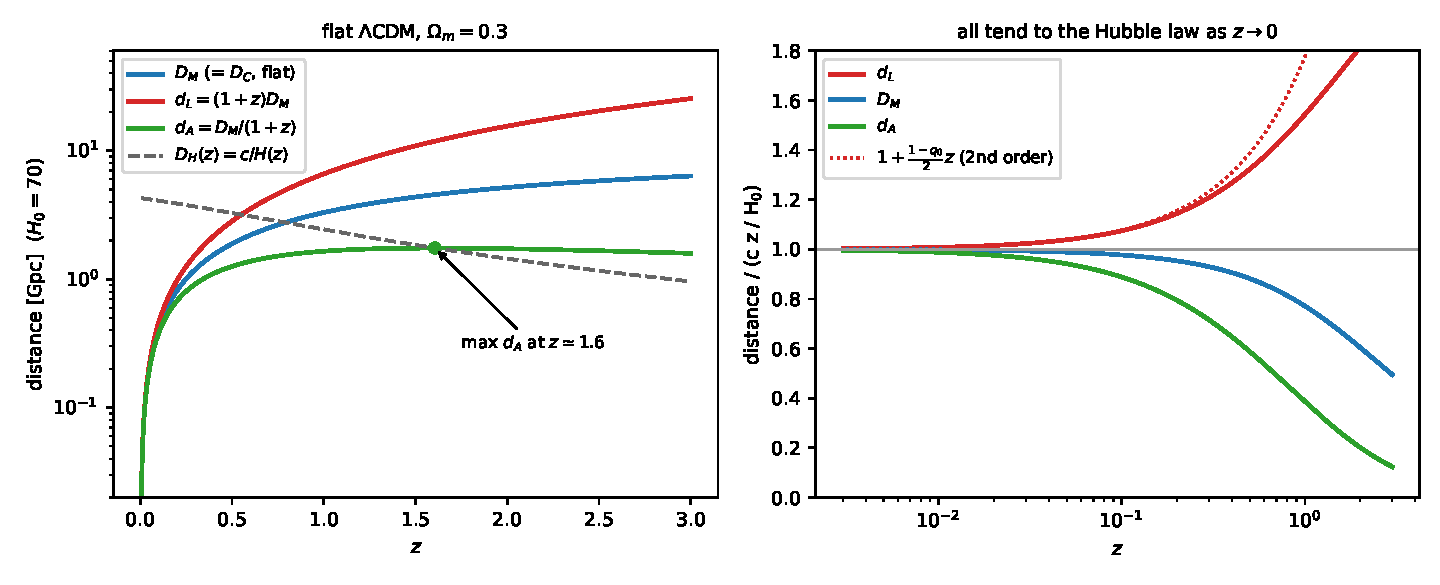
\includegraphics[width=0.95\textwidth]{figs/fig_dist_four.pdf}
\caption{\small ארבעת המרחקים ב-$\LCDM$ שטוח. $D_L$ עולה מהר, $D_A$ מגיע למקסימום ויורד, ו-$D_M$ שואף לאופק.}
\end{figure}

\begin{warnbox}
\textbf{מלכודות נפוצות.} (1) $v=cz$ נכון רק כש-$z\ll1$; ב-$z>1$ גלקסיות "בורחות" מהר מ-$c$ בלי סתירה ליחסות. (2) "מרחק" בלי לציין איזה --- חסר משמעות. (3) $D_M$ ולא $D_C$ הוא שנכנס ל-$D_A$ ול-$D_L$ כש-$k\neq0$.
\end{warnbox}

% ---------------------------------------------------------------------
\subsection*{תרגילים}
\begin{exercise}{גיל ותאוצה}
(א) חשבו את $t_0$ ב-\en{EdS} וב-$\LCDM$ שטוח עם $\Omega_m=0.3$, עבור $h=0.7$.
(ב) מצאו את ההסחה $z_{\rm acc}$ שבה $\ddot a=0$, ואת ההסחה שבה $\rho_m=\rho_\Lambda$. למה הן שונות?
(ג) מה $q_0$? מה הסימן שלו אומר?
\end{exercise}
\begin{solbox}
\textbf{פתרון.}
\textbf{(א)} זמן האבל: $1/H_0=977.8/h\,\Gyr=13.97\,\Gyr$ עבור $h=0.7$ (כי $1\,\Mpc/(1\,\kms)=977.8\,\Gyr$).
\begin{itemize}
\item \en{EdS}: $a\propto t^{2/3}\Rightarrow H=\frac{2}{3t}\Rightarrow t_0=\frac{2}{3H_0}=9.3\,\Gyr$.
\item $\LCDM$: מפתרון $\sinh$, בדרישה $a(t_0)=1$: $\sinh\!\big(\tfrac32\sqrt{\Omega_\Lambda}H_0t_0\big)=\sqrt{\Omega_\Lambda/\Omega_m}=1.528$. מכאן $\tfrac32\sqrt{0.7}\,H_0t_0=\mathrm{arsinh}(1.528)=1.210$, כלומר $H_0t_0=0.964$ ו-$t_0=13.5\,\Gyr$.
\end{itemize}
בדיקה: $t_0=H_0^{-1}\int_0^1\frac{da}{a\sqrt{\Omega_m a^{-3}+\Omega_\Lambda}}$ נותן אותו מספר נומרית. ה-$\Lambda$ "מאריך" את הגיל, כי בעבר ההתפשטות הייתה איטית יותר.

\textbf{(ב)} משוואת התאוצה עם $p_m=0$, $p_\Lambda=-\rho_\Lambda$:
\[
\frac{\ddot a}{a}=-\frac{4\pi G}{3}\big(\rho_m-2\rho_\Lambda\big)=0\ \Longrightarrow\ \rho_m=2\rho_\Lambda
\ \Longrightarrow\ \Omega_m(1+z)^3=2\Omega_\Lambda,
\]
\[
1+z_{\rm acc}=\Big(\frac{2\Omega_\Lambda}{\Omega_m}\Big)^{1/3}=\Big(\frac{1.4}{0.3}\Big)^{1/3}=1.67\ \Rightarrow\ z_{\rm acc}=0.67 .
\]
$\rho_m=\rho_\Lambda$: $(1+z)^3=\Omega_\Lambda/\Omega_m=2.33\Rightarrow z=0.33$. ההבדל: בתאוצה קובע $\rho+3p$, ולא $\rho$. ל-$\Lambda$ יש $\rho+3p=-2\rho$, ולכן "משקלו" כפול, והתאוצה מתחילה \emph{לפני} ש-$\Lambda$ שולט בצפיפות.

\textbf{(ג)} $q_0=\tfrac12\Omega_m-\Omega_\Lambda=0.15-0.70=-0.55$. $q_0<0\iff\ddot a>0$: היקום מאיץ היום. ב-\en{EdS} $q_0=+\tfrac12$ (מאט).
\end{solbox}

\begin{exercise}{המקסימום של $D_A$}
ב-\en{EdS}: (א) הראו ש-$D_C=\frac{2c}{H_0}\big(1-(1+z)^{-1/2}\big)$. (ב) מצאו את $z$ שבו $D_A$ מקסימלי ואת ערכו. (ג) גלקסיה בקוטר $30\,\kpc$: מה גודלה הזוויתי המינימלי (עבור $h=0.7$)?
\end{exercise}
\begin{solbox}
\textbf{פתרון.}
\textbf{(א)} ב-\en{EdS} $E(z)=(1+z)^{3/2}$:
\[
D_C=\frac{c}{H_0}\int_0^z(1+z')^{-3/2}dz'=\frac{c}{H_0}\Big[-2(1+z')^{-1/2}\Big]_0^z=\frac{2c}{H_0}\Big(1-\frac{1}{\sqrt{1+z}}\Big).
\]
ב-$z\to\infty$: $D_C\to2c/H_0$ --- זה אופק החלקיק היום.

\textbf{(ב)} $D_A=D_C/(1+z)$ (שטוח). נציב $u\equiv(1+z)^{-1/2}$, כך ש-$1/(1+z)=u^2$:
\[
D_A=\frac{2c}{H_0}\,u^2(1-u),\qquad \frac{d}{du}\big(u^2-u^3\big)=2u-3u^2=0\ \Rightarrow\ u=\frac23 .
\]
מכאן $1+z=9/4$, כלומר $z=1.25$, ו-
\[
D_A^{\max}=\frac{2c}{H_0}\cdot\frac49\cdot\frac13=\frac{8}{27}\frac{c}{H_0}=0.296\times4283\,\Mpc=1270\,\Mpc .
\]
\textbf{(ג)} $\theta=\ell/D_A\ge\ell/D_A^{\max}$:
\[
\theta_{\min}=\frac{30\,\kpc}{1270\,\Mpc}=2.4\times10^{-5}\ \text{רד'}=4.9'' .
\]
\emph{פירוש:} מעבר ל-$z=1.25$ גלקסיה נראית \emph{גדולה} יותר ככל שהיא רחוקה יותר. האור יצא כשהיקום היה קטן והגלקסיה הייתה קרובה אלינו. ב-$\LCDM$ המקסימום זז ל-$z\approx1.6$.
\end{solbox}

\begin{exercise}{מתי הקרינה שלטה?}
(א) מ-$\Omega_\gamma h^2=2.47\times10^{-5}$ ו-$\Omega_rh^2\simeq4.2\times10^{-5}$ (עם נייטרינו) ו-$\Omega_mh^2=0.143$, חשבו את $z_{\rm eq}$. (ב) מה הטמפרטורה של הקרינה אז ($T=T_0(1+z)$)? (ג) מצאו $a(t)$ ביקום של קרינה${}+$חומר בלבד בעזרת זמן קונפורמי $\eta$ ($dt=a\,d\eta$). רמז: $a(\eta)=a_{\rm eq}\big[(\eta/\eta_*)^2+2\eta/\eta_*\big]$.
\end{exercise}
\begin{solbox}
\textbf{פתרון.}
\textbf{(א)} $\rho_r\propto a^{-4}$ ו-$\rho_m\propto a^{-3}$, ולכן $\rho_r/\rho_m=(\Omega_r/\Omega_m)(1+z)$. שוויון:
\[
1+z_{\rm eq}=\frac{\Omega_m}{\Omega_r}=\frac{\Omega_mh^2}{\Omega_rh^2}=\frac{0.143}{4.2\times10^{-5}}\approx3400 .
\]
(היחס ב-$h^2$ מבטל את התלות ב-$H_0$. בלי נייטרינו היינו מקבלים 5800 --- הנייטרינו חשובים.)

\textbf{(ב)} $T=T_0(1+z)=2.7255\times3400\approx9300\,\mathrm K$, כלומר $k_BT\approx0.80\,\mathrm{eV}$.

\textbf{(ג)} עם $dt=a\,d\eta$ נסמן $a'=da/d\eta=a^2H$. משוואת פרידמן ($k=\Lambda=0$):
\[
a'^2=a^4H^2=H_0^2\big(\Omega_r+\Omega_m a\big).
\]
גוזרים לפי $\eta$: $2a'a''=H_0^2\Omega_m a'$, כלומר $a''=\tfrac12H_0^2\Omega_m=$ קבוע. אינטגרציה עם $a(0)=0$ ו-$a'(0)=H_0\sqrt{\Omega_r}$:
\[
a(\eta)=\frac{\Omega_mH_0^2}{4}\eta^2+\sqrt{\Omega_r}\,H_0\eta
=a_{\rm eq}\Big[\Big(\frac{\eta}{\eta_*}\Big)^2+2\frac{\eta}{\eta_*}\Big],\qquad
a_{\rm eq}=\frac{\Omega_r}{\Omega_m},\ \ \eta_*=\frac{2\sqrt{\Omega_r}}{\Omega_mH_0}.
\]
בדיקת גבולות: $\eta\ll\eta_*$: $a\propto\eta$, ו-$t=\int a\,d\eta\propto\eta^2$, ולכן $a\propto t^{1/2}$ (קרינה). $\eta\gg\eta_*$: $a\propto\eta^2$, $t\propto\eta^3$, ולכן $a\propto t^{2/3}$ (חומר). השוויון $a=a_{\rm eq}$ ב-$\eta/\eta_*=\sqrt2-1$.
\end{solbox}

% =====================================================================
\lecture{2}{\en{MCMC} וסופרנובות: מדידת האנרגיה האפלה}{שעתיים: חלק א' (שעה, סוף מפגש 1) --- בייס ו-\en{MCMC} על קו ישר; חלק ב' (שעה, מפגש 2) --- \en{Pantheon+} והמחברת \en{MCMC\_Pantheon\_he}.}
% =====================================================================

\begin{goalbox}
\textbf{מטרות.} (1) לנסח הסקה בייסיאנית: נראות, מוקדמת, מאוחרת, מרג'ינליזציה. (2) להבין את \en{Metropolis--Hastings} ו-\en{emcee}, ולדעת מתי מותר להאמין לשרשרת. (3) להחיל את אותה מכונה על 1590 סופרנובות ולמדוד $\Omega_m$ ו-$w$.
\end{goalbox}

\subsection*{חלק א' --- הסקה בייסיאנית ו-\en{MCMC}}

\subsection{משפט בייס}
\begin{equation}
\underbrace{P(\boldsymbol\theta|D)}_{\text{מאוחרת}}=\frac{\overbrace{\mathcal L(D|\boldsymbol\theta)}^{\text{נראות}}\ \overbrace{\pi(\boldsymbol\theta)}^{\text{מוקדמת}}}{\underbrace{P(D)}_{\text{עדות}}},
\qquad
\mathcal L\propto e^{-\chi^2/2},\quad \chi^2=\mathbf r^{\!\top}\mathsf C^{-1}\mathbf r,\quad \mathbf r=\mathbf d-\mathbf m(\boldsymbol\theta).
\end{equation}
למה בייס בקוסמולוגיה? יש יקום אחד, ואי אפשר לחזור על הניסוי. שואלים "מה סביר לגבי $\boldsymbol\theta$ בהינתן הנתונים", ולא "מה היה קורה בחזרות".

\textbf{מרג'ינליזציה.} תוצאה לפרמטר אחד מתקבלת באינטגרציה על כל השאר: $P(\theta_1|D)=\int P(\boldsymbol\theta|D)\,d\theta_2\cdots d\theta_n$. \emph{לא} מקבעים פרמטרי מטרד: אם $\rho$ הקורלציה בין שני פרמטרים, קיבוע אחד מהם מקטין את השגיאה על השני בפקטור $\sqrt{1-\rho^2}$ --- הערכת-חסר של השגיאה.

\subsection{למה לדגום, ואיך}
ב-$n$ פרמטרים רשת של 100 נקודות לציר עולה $100^n$ חישובי נראות. במקום זה יוצרים \textbf{שרשרת} של נקודות שהצפיפות שלהן פרופורציונלית למאוחרת; אז כל אינטגרל הוא ממוצע על הדגימות, וכל היסטוגרמה היא התפלגות שולית.

\begin{keybox}
\textbf{\en{Metropolis--Hastings}.} מנקודה $\boldsymbol\theta$:
\begin{enumerate}
\item מציעים $\boldsymbol\theta'=\boldsymbol\theta+\boldsymbol\epsilon$ (הצעה סימטרית, למשל גאוסית).
\item מחשבים $\alpha=\min\!\big[1,\;P(\boldsymbol\theta'|D)/P(\boldsymbol\theta|D)\big]$.
\item מקבלים את $\boldsymbol\theta'$ בהסתברות $\alpha$; אחרת \emph{חוזרים על} $\boldsymbol\theta$ בשרשרת.
\end{enumerate}
רק \emph{יחס} מאוחרות נכנס, ולכן העדות $P(D)$ לא נחוצה. שיווי משקל מפורט מבטיח שהשרשרת מתכנסת למאוחרת.
\end{keybox}
\textbf{\en{emcee}} (\en{Goodman--Weare}): אנסמבל של "הולכים"; כל הולך מציע צעד לאורך הקו אל הולך אחר (\en{stretch move}). הדוגם אינווריאנטי תחת טרנספורמציות אפיניות, ולכן מסתדר עם מאוחרות צרות ומשופעות בלי כיוונון גודל צעד.

\textbf{אבחון --- לפני שמדווחים מספר:}
\begin{itemize}
\item \textbf{\en{burn-in}:} השלכת החלק הראשון ($\sim5\tau$), שתלוי בנקודת ההתחלה.
\item \textbf{זמן אוטוקורלציה $\tau$:} $N_{\rm eff}\approx N_{\rm steps}N_{\rm walkers}/\tau$. דורשים שרשרת באורך $\gtrsim50\tau$.
\item \textbf{\en{Gelman--Rubin}:} $\hat R=\sqrt{[\tfrac{n-1}{n}W+(1+\tfrac1M)B]/W}$ מ-$M$ ריצות; $\hat R-1<0.01$.
\item שיעור קבלה $0.2$--$0.7$. קבלה גבוהה אינה הצלחה: צעדים זעירים מתקבלים תמיד.
\end{itemize}

\textbf{\en{corner plot}.} באלכסון: התפלגויות שוליות (חציון ו-$16/84$ אחוזונים $=\pm1\sigma$). מחוץ לאלכסון: קווי מתאר דו-ממדיים. אליפסה משופעת $=$ קורלציה; "בננה" $=$ מאוחרת לא גאוסית, ואז $\pm$ ו-$\rho$ לא מספיקים.

\textbf{השוואת מודלים.} $\mathrm{AIC}=\chi^2_{\min}+2k$, \ $\mathrm{BIC}=\chi^2_{\min}+k\ln N$; בקירוב $\ln B_{12}\simeq-\Delta\mathrm{BIC}/2$. פרמטר נוסף משתלם רק אם $\Delta\chi^2\gtrsim2$ (\en{AIC}) או $\gtrsim\ln N$ (\en{BIC}).

\begin{figure}[htbp]\centering
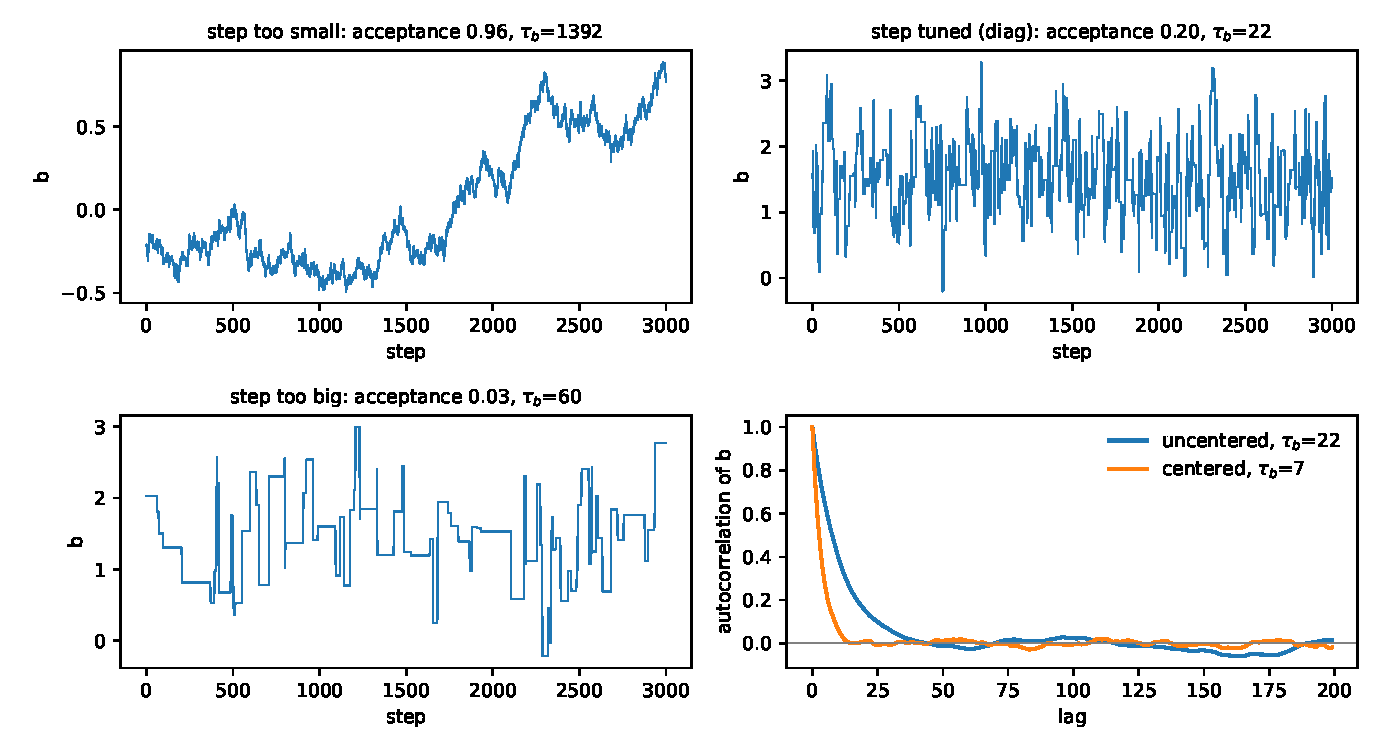
\includegraphics[width=0.49\textwidth]{figs/fig_line_mcmc.pdf}\hfill
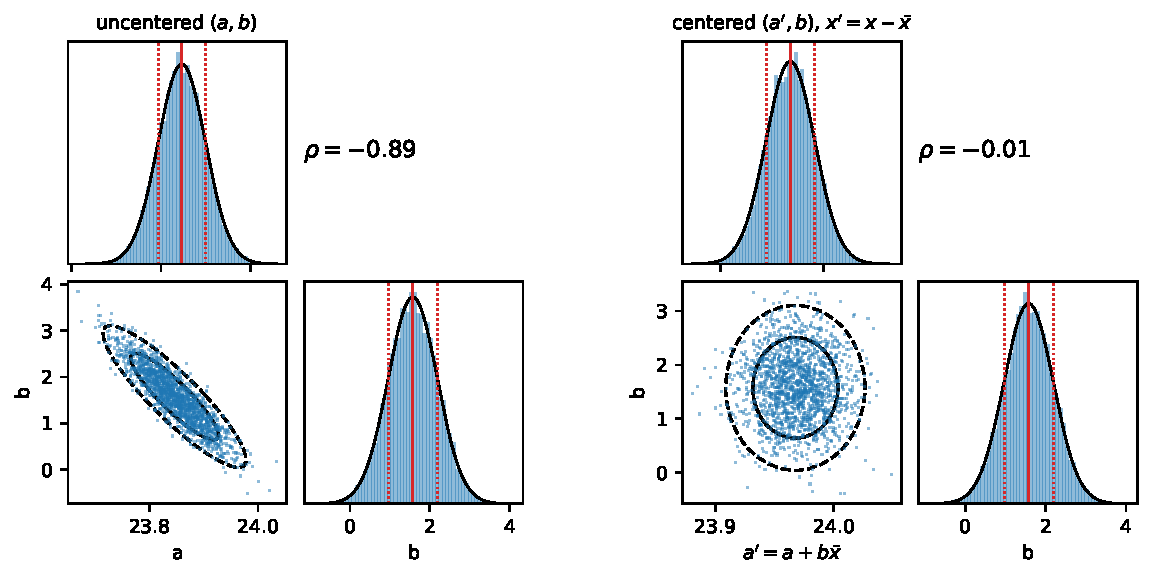
\includegraphics[width=0.42\textwidth]{figs/fig_line_corner.pdf}
\caption{\small קו ישר: עקבות השרשרת (שמאל) ו-\en{corner plot} (ימין). הדגימה משחזרת את הפתרון האנליטי, כולל $\rho_{ab}\approx-0.9$.}
\end{figure}

\subsection*{חלק ב' --- סופרנובות ואנרגיה אפלה}

\subsection{נר תקני}
סופרנובה \en{Ia}: ננס לבן שמתקרב לגבול צ'נדרסקאר ומתפוצץ. לאחר תיקוני מתיחה (\en{stretch}, $x_1$) וצבע ($c$) הבהירות בשיא אחידה ל-$\sim0.1$ מג'. מודול המרחק:
\begin{equation}
m_B=M_B+\mu(z),\qquad \mu=5\log_{10}\frac{D_L}{10\,\mathrm{pc}}=5\log_{10}\frac{D_L}{\Mpc}+25 .
\end{equation}
כותבים $D_L=(c/H_0)\,\hat D_L(z;\Omega_m,w)$. אז
\begin{equation}
m_B=\underbrace{M_B+5\log_{10}\!\Big(\frac{c/H_0}{\Mpc}\Big)+25}_{\mathcal M}+5\log_{10}\hat D_L(z;\boldsymbol\theta) .
\end{equation}
\begin{warnbox}
\textbf{$H_0$ ו-$M_B$ מופיעים רק בצירוף $\mathcal M$.} סופרנובות לבדן מודדות את \emph{צורת} $D_L(z)$, כלומר $\Omega_m,w$, ולא את $H_0$. כדי לקבל $H_0$ צריך לכייל את $M_B$ בעזרת צפייניים --- ושם נולד מתח האבל (הרצאה 5).
\end{warnbox}

\textbf{1998.} ב-$z=0.5$ ההפרש ב-$\mu$ בין \en{EdS} ל-$\LCDM$ הוא $\sim0.4$ מג': הסופרנובות הרחוקות \emph{חלשות} מהצפוי (תרגיל 2.3). זו התגלית (\en{Riess et al.\ 1998; Perlmutter et al.\ 1999}).

\subsection{מרג'ינליזציה אנליטית על $\mathcal M$}
$\mathcal M$ נכנס לינארית. עם $\mathbf r_0=\mathbf m_B-\boldsymbol\mu_{\rm th}$:
\begin{equation}
\chi^2(\mathcal M)=A-2\mathcal MB+\mathcal M^2S,\quad A=\mathbf r_0^{\!\top}\mathsf C^{-1}\mathbf r_0,\ \ B=\mathbf 1^{\!\top}\mathsf C^{-1}\mathbf r_0,\ \ S=\mathbf 1^{\!\top}\mathsf C^{-1}\mathbf 1 .
\end{equation}
אינטגרל גאוסי על $\mathcal M$ (מוקדמת אחידה) נותן
\begin{equation}
\boxed{\;\chi^2_{\rm marg}=A-\frac{B^2}{S}\;}\qquad(+\ \text{קבוע}),\qquad \hat{\mathcal M}=B/S .
\end{equation}
פרמטר אחד פחות לדגום, ושרשרת מהירה פי 2 (בדיקה בסעיף 19 במחברת).

\subsection{התוצאות}
\begin{center}\small
\begin{tabular}{@{}p{2.3cm}p{2.3cm}p{11.2cm}@{}}
\toprule
מודל & פרמטרים & תוצאה (\en{Pantheon+}, 1590 \en{SNe}, $z>0.01$) \\ \midrule
$\LCDM$ שטוח & $\Omega_m$ & $\Omega_m=0.332\pm0.018$, \ $\chi^2=1403$ ל-1589 ד"ח \\
$w$\en{CDM} שטוח & $\Omega_m,w$ & $\Omega_m=0.29^{+0.07}_{-0.08}$, $w=-0.90^{+0.14}_{-0.16}$, $\rho=-0.94$; $\Delta\mathrm{BIC}=+6.9$ לטובת $\Lambda$ \\
$\Lambda$ עקום & $\Omega_m,\Omega_\Lambda$ & $q_0=-0.47\pm0.06$ \ ($P(q_0<0)\approx1$), \ $\Omega_k=0.09\pm0.13$ \\ \bottomrule
\end{tabular}
\end{center}

\begin{figure}[htbp]\centering
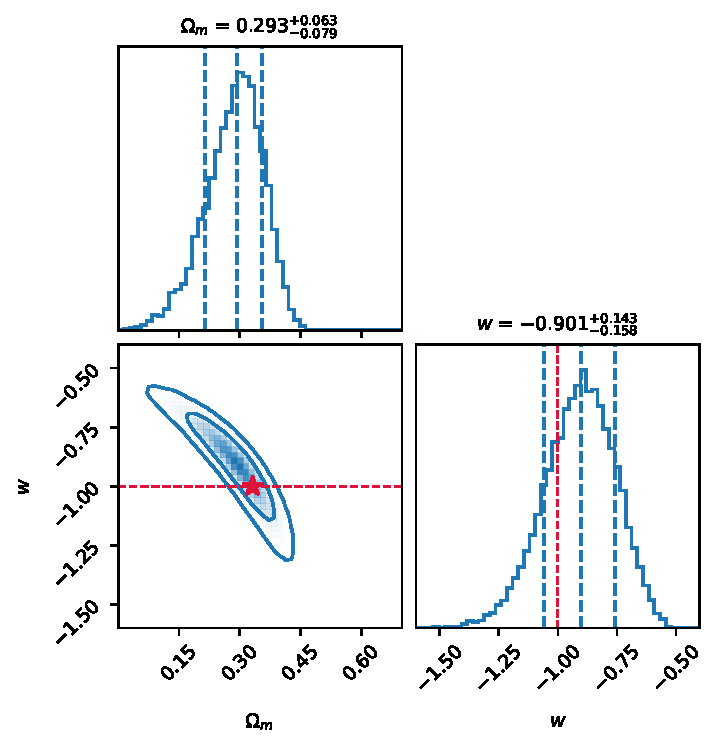
\includegraphics[width=0.38\textwidth]{figs/fig_pp_wcdm.pdf}\hfill
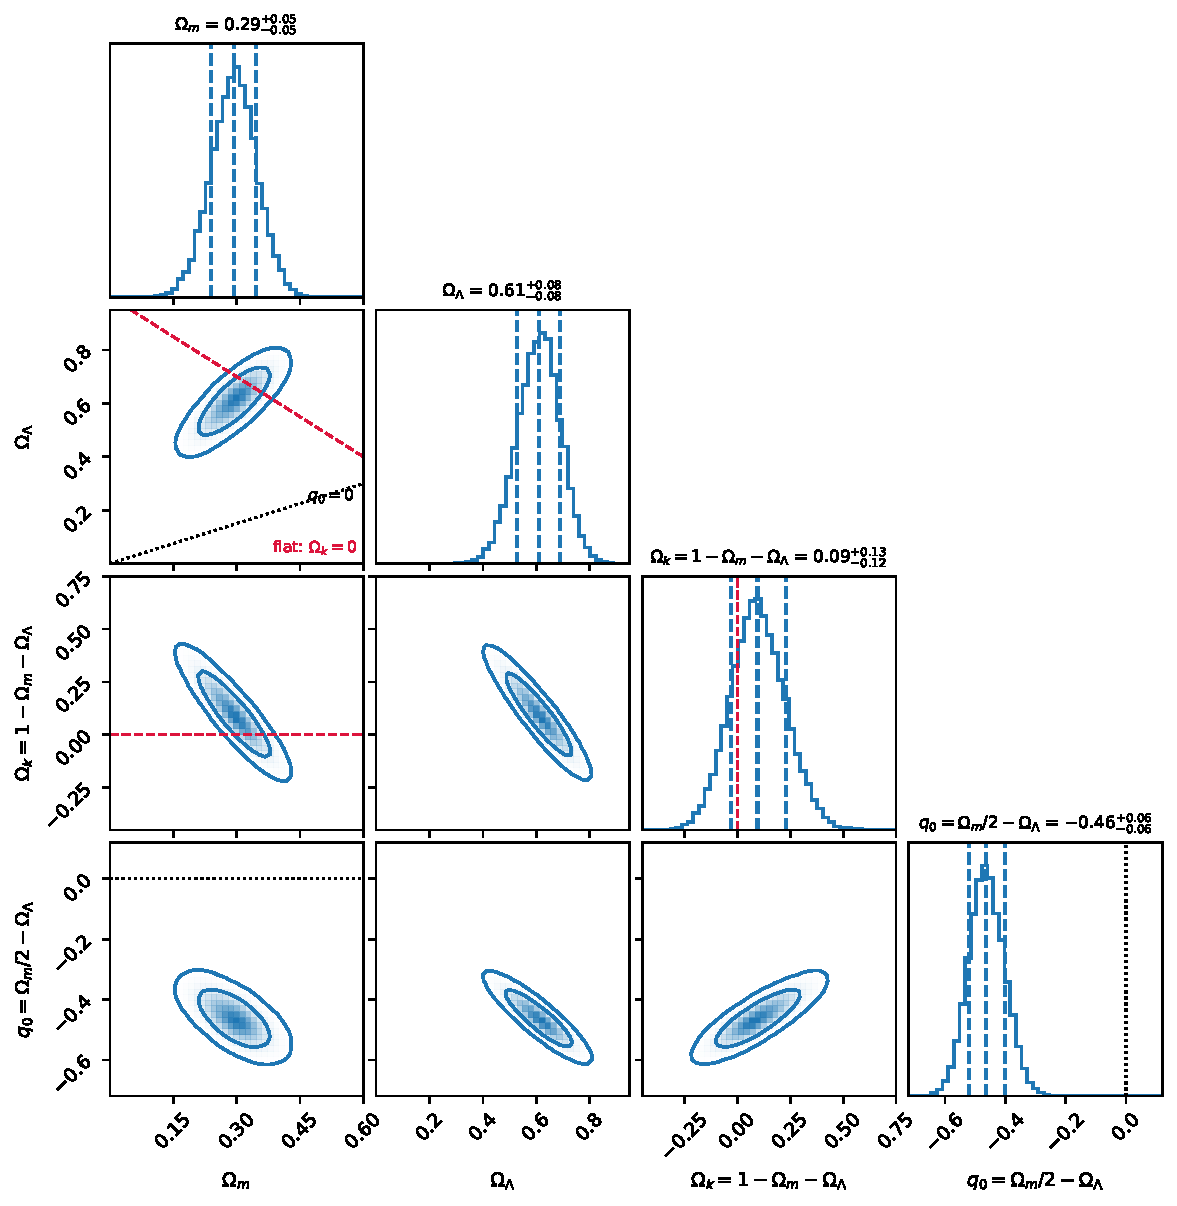
\includegraphics[width=0.40\textwidth]{figs/fig_pp_curved.pdf}
\caption{\small \en{Pantheon+}: ניוון $\Omega_m$--$w$ (שמאל) ומישור $\Omega_m$--$\Omega_\Lambda$ עם הפרמטרים הנגזרים $\Omega_k$, $q_0$ (ימין). התאוצה ($q_0<0$) איתנה; הערך של $\Omega_k$ לא.}
\end{figure}

\textbf{קריאה.} ($\Omega_m,w$): הנתונים מודדים צירוף אחד --- הגדלת $\Omega_m$ מפוצה בהקטנת $w$. ($\Omega_m,\Omega_\Lambda$): בטווח $z$ הנמוך מודדים בעיקר $q_0=\Omega_m/2-\Omega_\Lambda$. את הניוון שוברים עם \en{CMB} ו-\en{BAO} (הרצאה 5).

\subsection{סיור במחברת \en{MCMC\_Pantheon\_he}}
המחברת בונה את המכונה פעם אחת, על קו ישר שבו אפשר לבדוק הכול אנליטית, ואז מחליפה רק את המודל.
\begin{center}\small
\begin{tabular}{@{}p{2.2cm}p{5.3cm}p{7.2cm}@{}}
\toprule
סעיפים & מה קורה & מה להראות בכיתה \\ \midrule
1--2 & נתונים סינתטיים, פתרון אנליטי (מטריצת פישר $F=A^{\!\top}A/\sigma^2$) & $\rho_{ab}=-0.90$: הנתונים רחוקים מהראשית \\
3 & \texttt{log\_prior}, \texttt{log\_likelihood}, \texttt{log\_probability} & החזרת $-\infty$ $=$ "אסור"; למה לוגריתם \\
4--5 & איתחול 32 הולכים בכדור קטן סביב המקסימום; \texttt{run\_mcmc} & צורת השרשרת \texttt{(nsteps, nwalkers, ndim)} \\
6 & עקבות, $\tau\approx32$, \en{burn-in} $=5\tau$, $\hat R$ מ-4 ריצות & $N_{\rm eff}\approx5900$; $\hat R-1<10^{-3}$ \\
7--8 & \en{corner}; 60 קווים מהמאוחרת & הדגימה $=$ האנליטי; ה"צוואר" ב-$\bar x$ \\
9--10 & מרכוז $x'=x-\bar x$; קיבוע מול מרג'ינליזציה & קיבוע מקטין $\sigma_b$ פי $2.34=1/\sqrt{1-\rho^2}$ \\
11 & קו מול פרבולה: \en{AIC/BIC} & $\Delta\mathrm{BIC}=+3.1$: הקו מספיק \\ \midrule
12--13 & \en{Pantheon+}: \texttt{zHD}, \texttt{zHEL}, \texttt{m\_b\_corr}, מטריצת שונות מלאה & הופכים את $\mathsf C$ \emph{פעם אחת} לפני הריצה \\
14 & $\mu(z)$ על רשת $z$ צפופה + \texttt{np.interp} & מהיר פי מאות מ-\texttt{quad} לכל סופרנובה \\
15 & $\chi^2_{\rm marg}=A-B^2/S$ & \en{EdS}: $\chi^2=2101$; $\LCDM$: $1403$ \\
16 & $\LCDM$: רשת מול \en{emcee} & $\Omega_m=0.332\pm0.018$ בשתי הדרכים \\
17 & $w$\en{CDM} & בננה, $\rho=-0.94$, $P(w<-1)=0.27$ \\
18 & עקום; פרמטרים נגזרים שורה-שורה & $q_0<0$ בלי "התפשטות שגיאות" \\
19 & דגימה מפורשת של $\mathcal M$ & אותה תוצאה; $\tau$ גדל פי 2 \\ \bottomrule
\end{tabular}
\end{center}

הלב של כל הניתוח --- שלוש פונקציות קצרות:
\begin{otherlanguage}{english}
\begin{lstlisting}
def chi2_marg(mu):                      # analytic marginalisation over M
    r0 = mb - mu
    A = r0 @ (Cinv @ r0); B = s_vec @ r0   # s_vec = Cinv@1, S_sum = 1^T Cinv 1
    return A - B*B/S_sum

def log_prob_wcdm(theta):
    Om, w = theta
    if not (0 < Om < 1 and -3 < w < 0): return -np.inf    # flat prior
    mu = mu_model(Om, w)
    return -np.inf if mu is None else -0.5*chi2_marg(mu)

sampler = emcee.EnsembleSampler(32, 2, log_prob_wcdm)
sampler.run_mcmc(best + 1e-2*rng.normal(size=(32, 2)), 4000)
\end{lstlisting}
\end{otherlanguage}

% ---------------------------------------------------------------------
\subsection*{תרגילים}
\begin{exercise}{קו ישר אנליטית}
$N$ נקודות $y_i=a+bx_i$ עם שגיאה $\sigma$. (א) כתבו את $\chi^2$ והראו שמטריצת פישר היא $F=\frac{N}{\sigma^2}\begin{pmatrix}1&\bar x\\ \bar x&\overline{x^2}\end{pmatrix}$. (ב) הראו ש-$\rho_{ab}=-\bar x/\sqrt{\overline{x^2}}$. (ג) הראו שהשגיאה השולית על $b$ גדולה מהשגיאה המותנית (כש-$a$ מקובע) בפקטור $1/\sqrt{1-\rho^2}$. מה זה אומר על תכנון סקר סופרנובות?
\end{exercise}
\begin{solbox}
\textbf{פתרון.}\ (א) $F_{ij}=\tfrac12\partial_i\partial_j\chi^2$: $F_{aa}=N/\sigma^2$, $F_{ab}=N\bar x/\sigma^2$, $F_{bb}=N\overline{x^2}/\sigma^2$.\\
(ב) ל-$2\times2$, $C=F^{-1}$ ו-$\rho=C_{ab}/\sqrt{C_{aa}C_{bb}}=-F_{ab}/\sqrt{F_{aa}F_{bb}}=-\bar x/\sqrt{\overline{x^2}}$.\\
(ג) $\sigma_b^2(\text{שולי})=C_{bb}=F_{aa}/\det F$, $\sigma_b^2(\text{מותנה})=1/F_{bb}$. היחס: $F_{aa}F_{bb}/\det F=1/(1-\rho^2)$. בסקר: זרוע ארוכה בהסחה, ומדגם עוגן ב-$z$ נמוך, כדי לשבור את הקורלציה עם ההיסט $\mathcal M$. (במחברת: $\rho=-0.90$, יחס $2.34$.)
\end{solbox}

\begin{exercise}{מרג'ינליזציה על ההיסט}
(א) בצעו את האינטגרל $\int e^{-\chi^2(\mathcal M)/2}d\mathcal M$ עם $\chi^2=A-2\mathcal MB+\mathcal M^2S$ והראו ש-$\chi^2_{\rm marg}=A-B^2/S+\ln(S/2\pi)$. (ב) הראו שזה שווה (עד קבוע) ל-$\chi^2$ המינימלי על $\mathcal M$ (\en{profile}). למה זה נכון כאן ולא באופן כללי? (ג) כש-$\mathsf C$ אלכסונית, מה $\hat{\mathcal M}$?
\end{exercise}
\begin{solbox}
\textbf{פתרון.}\ (א) השלמה לריבוע: $\chi^2=S(\mathcal M-B/S)^2+A-B^2/S$. האינטגרל הגאוסי נותן $\sqrt{2\pi/S}\,e^{-(A-B^2/S)/2}$, ולכן $-2\ln=A-B^2/S+\ln(S/2\pi)$.\\
(ב) המינימום על $\mathcal M$ ב-$\hat{\mathcal M}=B/S$ נותן בדיוק $A-B^2/S$. השוויון נובע מכך שהנראות גאוסית בפרמטר לינארי, $S$ לא תלוי ב-$\boldsymbol\theta$ (מטריצת שונות קבועה) והמוקדמת אחידה. בפרמטר לא-לינארי, או כש-$\mathsf C$ תלויה בפרמטרים, מרג'ינליזציה ופרופיל שונים (הבדל "נפח").\\
(ג) $\hat{\mathcal M}=\sum_i(r_{0,i}/\sigma_i^2)\big/\sum_i\sigma_i^{-2}$: ממוצע משוקלל של השאריות.
\end{solbox}

\begin{exercise}{כמה חלשות הסופרנובות?}
(א) חשבו $\Delta\mu=\mu_{\LCDM}-\mu_{\rm EdS}$ ב-$z=0.5$ עבור $\Omega_m=0.3$ (אינטגרל נומרי פשוט, או סימפסון בשלוש נקודות). (ב) עם פיזור $0.15$ מג' לסופרנובה, כמה סופרנובות ב-$z\approx0.5$ נחוצות כדי להבחין בין המודלים ב-$5\sigma$? (ג) למה מספיק לדעת את $\Delta\mu$ ולא את $H_0$?
\end{exercise}
\begin{solbox}
\textbf{פתרון.}\ (א) $\int_0^{0.5}dz/E=0.441$ ($\LCDM$) מול $2(1-1.5^{-1/2})=0.367$ (\en{EdS}). $\Delta\mu=5\log_{10}(0.441/0.367)=+0.40$ מג': ב-$\LCDM$ הסופרנובות חלשות יותר.\\
(ב) $\mathcal M$ לא ידוע, ולכן משווים ממוצע ב-$z\approx0.5$ לממוצע ב-$z$ נמוך: $\sigma_{\Delta}=0.15\sqrt{2/N}<0.40/5$ נותן $N\gtrsim7$ בכל סל. בפועל השגיאות השיטתיות (כיול, אבק, אבולוציה) $\sim0.02$--$0.03$ מג' הן הגבול, לא $N$.\\
(ג) $H_0$ מוסיף קבוע ל-$\mu$ בכל $z$. ההבחנה היא בצורת $\mu(z)$, יחסית ל-$z$ נמוך.
\end{solbox}

% =====================================================================
\lecture{3}{חומר אפל והרשת הקוסמית: הפרעות לינאריות ואורך ג'ינס}{מפגש 2, כשעה ורבע. \ (5' הבעיה, 20' גזירה ניוטונית, 25' \en{GR} ופתרונות מעל האופק, 5' רשת קוסמית, תרגילים)}
% =====================================================================

\begin{goalbox}
\textbf{מטרות.} (1) לגזור את משוואת הצמיחה הלינארית מהידרודינמיקה ניוטונית ביקום מתפשט. (2) לקבל ממנה את אורך ג'ינס ולהבין למה בריונים לבדם לא מספיקים. (3) לגזור את ההפרעות מ-\en{GR} בכיול הניוטוני, להראות שמתקבלת אותה משוואת צמיחה בדיוק (לצפיפות הקומובילית), ולפתור מעל האופק בעידני החומר והקרינה. (4) ממבנה לינארי לרשת: \en{Zel'dovich} וקריסה כדורית.
\end{goalbox}

\subsection{הבעיה}
ב-\en{CMB}: $\delta T/T\sim10^{-5}$, ולכן $\delta\equiv\delta\rho/\bar\rho\sim10^{-5}$ ב-$z\approx1100$. היום: גלקסיות עם $\delta\sim10^{6}$ וצבירים עם $\delta\sim200$. איך צומחים פקטור $\gtrsim10^5$?

\subsection{גזירה ניוטונית}
\textbf{משוואות.} רציפות, אוילר ופואסון לנוזל עם צפיפות $\rho$, מהירות $\mathbf V$, לחץ $p$:
\begin{equation}
\partial_t\rho+\nabla\!\cdot(\rho\mathbf V)=0,\qquad
\partial_t\mathbf V+(\mathbf V\!\cdot\!\nabla)\mathbf V=-\nabla\Phi-\frac{\nabla p}{\rho},\qquad
\nabla^2\Phi=4\pi G\rho .
\end{equation}
\textbf{רקע.} $\rho=\bar\rho(t)$, $\mathbf V=H\mathbf r$. רציפות: $\bar\rho\propto a^{-3}$. אוילר ופואסון: $\ddot a/a=-\tfrac{4\pi G}{3}\bar\rho$ --- משוואת פרידמן לחומר. \emph{הרקע הוא יקום פרידמן; לא הנחנו זאת.}

\begin{warnbox}
\textbf{ג'ינס במדיום סטטי} (1902): $\nabla^2\Phi_0=4\pi G\rho_0\neq0$ עם $\Phi_0=$ קבוע --- סתירה, שג'ינס "התעלם" ממנה (\en{Jeans swindle}). ביקום מתפשט אין סתירה: $\Phi_0=-\tfrac12(\ddot a/a)r^2$ פותר את פואסון. ההתפשטות היא שמצדיקה את החישוב.
\end{warnbox}

\textbf{הפרעות.} $\rho=\bar\rho(1+\delta)$, $\mathbf V=H\mathbf r+\mathbf u$, $\Phi=\Phi_0+\phi$, $\delta p=c_s^2\bar\rho\delta$. בקואורדינטות נעות $\mathbf x=\mathbf r/a$ (אז $\nabla_r=a^{-1}\nabla_x$), סדר ראשון:
\begin{equation}
\dot\delta+\frac1a\nabla\!\cdot\mathbf u=0,\qquad
\dot{\mathbf u}+H\mathbf u=-\frac1a\nabla\phi-\frac{c_s^2}{a}\nabla\delta,\qquad
\nabla^2\phi=4\pi G\bar\rho a^2\delta .
\end{equation}
האיבר $H\mathbf u$ הוא "חיכוך האבל": בלי כוחות $\mathbf u\propto1/a$. נגזרת זמן של הראשונה, דיברגנץ של השנייה, הצבה, ומעבר לפורייה ($\nabla^2\to-k^2$, $k$ נע):
\begin{equation}
\boxed{\;\ddot\delta_k+2H\dot\delta_k=\Big(4\pi G\bar\rho-\frac{c_s^2k^2}{a^2}\Big)\delta_k\;}
\label{eq:growth}
\end{equation}
מתנד מרוסן שבו "קבוע הקפיץ" מחליף סימן. כל מוד $k$ מתפתח בנפרד --- רק בתורה הלינארית.

\subsection{אורך ג'ינס}
הכבידה מנצחת את הלחץ כאשר $k<k_J$:
\begin{equation}
\boxed{\;k_J=\frac{a\sqrt{4\pi G\bar\rho}}{c_s},\qquad
\lambda_J=\frac{2\pi a}{k_J}=c_s\sqrt{\frac{\pi}{G\bar\rho}},\qquad
M_J=\frac{4\pi}{3}\bar\rho\Big(\frac{\lambda_J}{2}\Big)^3\;}
\end{equation}
\begin{itemize}
\item $\lambda>\lambda_J$: צמיחה. \quad $\lambda<\lambda_J$: גלי קול (תנודות אקוסטיות --- הבסיס של הרצאה 5).
\item פיזיקלית: $\lambda_J\sim c_s\,t_{\rm ff}$ --- המרחק שגל קול עובר בזמן נפילה חופשית $t_{\rm ff}\sim(G\rho)^{-1/2}$.
\end{itemize}

\begin{figure}[htbp]\centering
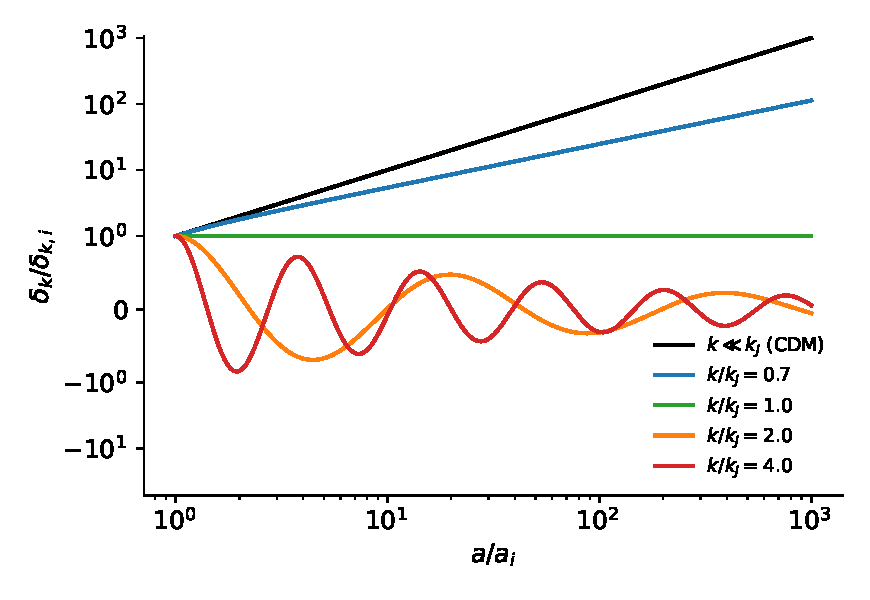
\includegraphics[width=0.55\textwidth]{figs/fig_jeans.pdf}
\caption{\small פתרון נומרי של \eqref{eq:growth} ב-\en{EdS} עבור יחס קבוע $k/k_J$. מתחת ל-$k_J$ ההפרעה צומחת; מעליו היא מתנודדת ודועכת.}
\end{figure}

\subsection{פתרונות, ולמה צריך חומר אפל}
\begin{keybox}
\textbf{\en{EdS}, $c_s=0$:} $4\pi G\bar\rho=\frac{2}{3t^2}$, $H=\frac{2}{3t}$. הצבת $\delta\propto t^n$: $3n^2+n-2=0$, ולכן
\begin{equation}
\delta_+\propto t^{2/3}\propto a,\qquad \delta_-\propto t^{-1}.
\end{equation}
הצמיחה היא \emph{חזקה} של $a$, לא מעריכית. ב-$\Lambda$: $\bar\rho\to0$ ו-$\delta\to$ קבוע. בעידן הקרינה (מתחת לאופק): $\delta_m\propto\ln a$ (\en{Mészáros}) --- הקרינה מגדילה את $H$ אבל לא מתקבצת.
\end{keybox}
\textbf{הטיעון.} בריונים צמודים לפוטונים עד $z\approx1100$: $c_s\approx c/\sqrt3$ ו-$M_J\sim10^{17}\Msun$, יותר ממסת האופק (תרגיל 3.1). הם מתחילים לצמוח רק ב-$z\approx1100$, ועד היום מקבלים פקטור $\lesssim1100$:
\begin{equation}
10^{-5}\times10^{3}=10^{-2}\ll1 .
\end{equation}
\emph{לא היו גלקסיות.} חומר שאינו מצומד לפוטונים צומח כבר מ-$z_{\rm eq}\approx3400$ (ולוגריתמית לפני כן), ואחרי הרקומבינציה הבריונים נופלים לבורות מוכנים.

\textbf{חם או קר?} חלקיקים מהירים זורמים החוצה מבורות (\en{free streaming}): בסולמות מתחת ל-$\lambda_{\rm fs}\sim\int v\,dt/a$ ההפרעות נמחקות. לנייטרינו ($m\sim\mathrm{eV}$) $\lambda_{\rm fs}\sim100\,\Mpc$: מבנה גדול נוצר ראשון ומתפרק (\en{top-down}), בניגוד לתצפית שגלקסיות זקנות מצבירים. לכן החומר האפל \textbf{קר}: $v\ll c$ מאז ההתנתקות, מבנה נבנה מלמטה למעלה (\en{bottom-up}).

\textbf{קצב הצמיחה.} $f\equiv d\ln D/d\ln a\simeq\Omega_m(a)^{0.55}$ ב-\en{GR}. נמדד מעיוותי מרחב-הסחה (\en{RSD}) כ-$f\sigma_8$, מבחן ישיר לכבידה.

\subsection{הגזירה היחסותית: מהמטריקה ועד משוואת הצמיחה}
הגזירה הניוטונית הניחה פואסון ומהירויות קטנות. כאן לא מניחים כבידה ניוטונית: מפריעים את \emph{המטריקה}, מחשבים את העקמומיות, ומשווים ל-$T^\mu{}_\nu$, בדיוק כמו בגזירת משוואות פרידמן בהרצאה 1. החשבון ארוך, אבל לכל רכיב של המשוואות יש תפקיד אחד:
\begin{center}\small
\begin{tabular}{@{}lll@{}}
\toprule
משוואה & סוג & מה היא נותנת \\ \midrule
רכיב $00$ של איינשטיין & אילוץ & פואסון יחסותי: $\Phi\leftrightarrow\delta$ \\
רכיב $0i$ & אילוץ & $\Phi'\leftrightarrow$ זרימת החומר $\theta$ \\
רכיב $ij$ חסר עקבה & אילוץ & $\Phi=\Psi$ \\
רכיב $ij$ עקבה & דינמי & התפתחות $\Phi$ (לא עצמאי כשיש רק אבק) \\
$\nabla_\mu T^\mu{}_0=0$ & שימור & רציפות: התפתחות $\delta$ \\
$\nabla_\mu T^\mu{}_i=0$ & שימור & אוילר: התפתחות $\theta$ \\ \bottomrule
\end{tabular}
\end{center}

\textbf{שלב 0: הרקע בזמן קונפורמי.} $d\eta=dt/a$, $ds^2=a^2(\eta)(-d\eta^2+d\mathbf x^2)$, $'\equiv d/d\eta$, $\mathcal H\equiv a'/a=aH$. משוואות פרידמן (שטוח) הופכות ל-
\begin{equation}
\begin{gathered}
\mathcal H^2=\frac{8\pi G}{3}a^2\rho,\qquad \mathcal H'=-\frac{4\pi G}{3}a^2(\rho+3p),\qquad \rho'=-3\mathcal H(\rho+p),\\
\Rightarrow\qquad \mathcal H^2-\mathcal H'=4\pi Ga^2(\rho+p).
\end{gathered}
\label{eq:gr-bg}
\end{equation}
($\Lambda$ היא נוזל עם $p=-\rho$, ולכן לא תורמת ל-$\rho+p$.) בעידן החומר $a\propto\eta^2$, $\mathcal H=2/\eta$; בעידן הקרינה $a\propto\eta$, $\mathcal H=1/\eta$.

\textbf{שלב 1: המטריקה המופרעת וחופש הכיול.} להפרעה כללית יש חלקים סקלריים (קשורים לצפיפות), וקטוריים (דועכים) וטנזוריים (גלי כבידה, הרצאה 6), שבסדר ראשון אינם מתערבבים. לחלק הסקלרי ארבע פונקציות, אבל טרנספורמציית קואורדינטות $x^\mu\to x^\mu+\xi^\mu$ (שתי פונקציות סקלריות) מסלקת שתיים. הבחירה הנוחה היא \textbf{הכיול הניוטוני}:
\begin{equation}
\boxed{\;ds^2=a^2(\eta)\big[-(1+2\Psi)\,d\eta^2+(1-2\Phi)\,\delta_{ij}dx^idx^j\big]\;},\qquad|\Phi|,|\Psi|\ll1 .
\end{equation}
$\Psi$ משנה את קצב השעון המקומי (הפוטנציאל הניוטוני); $\Phi$ משנה את העקמומיות המרחבית. ב-\en{CMB} $|\Phi|\sim10^{-5}$.

\begin{warnbox}
\textbf{$\delta$ תלויה בכיול.} שינוי כיול מזיז את משטחי $t=$ קבוע, ולכן משנה את $\delta\rho/\rho$ באיבר מסדר $3\mathcal H\theta/k^2$. מתחת לאופק ($k\gg\mathcal H$) זה זניח; מעל האופק זה מכריע. לכן מעל האופק צריך לבחור גודל שאינו תלוי בכיול (להלן: $\Delta$ ו-$\mathcal R$).
\end{warnbox}

\textbf{שלב 2: סמלי כריסטופל} (סדר ראשון; אפס הסדר הוא של הרצאה 1):
\begin{align}
\Gamma^0_{00}&=\mathcal H+\Psi', & \Gamma^0_{0i}&=\Gamma^i_{00}=\partial_i\Psi, & \Gamma^0_{ij}&=\big[\mathcal H-2\mathcal H(\Phi+\Psi)-\Phi'\big]\delta_{ij},\notag\\
\Gamma^i_{0j}&=(\mathcal H-\Phi')\,\delta^i_j, & \Gamma^i_{jk}&=-\big(\delta^i_j\partial_k\Phi+\delta^i_k\partial_j\Phi-\delta_{jk}\partial_i\Phi\big). &&
\end{align}
למשל $\Gamma^0_{ij}=-\tfrac12g^{00}\partial_0g_{ij}=(1-2\Psi)\big[\mathcal H(1-2\Phi)-\Phi'\big]\delta_{ij}$. ההפרעה מוסיפה רק נגזרות זמן של הפוטנציאלים ו"כוחות" (גרדיאנטים).

\textbf{שלב 3: העקמומיות.} מציבים בטנזור ריצ'י ומרכיבים $G^\mu{}_\nu$ (חשבון ארוך; כדאי לבדוק סימבולית):
\begin{align}
a^2\,\delta G^0{}_0&=-2\nabla^2\Phi+6\mathcal H(\Phi'+\mathcal H\Psi),\notag\\
a^2\,\delta G^0{}_i&=-2\,\partial_i(\Phi'+\mathcal H\Psi),\notag\\
a^2\,\delta G^i{}_j&=\delta^i_j\big[2\Phi''+2\mathcal H(\Psi'+2\Phi')+2(2\mathcal H'+\mathcal H^2)\Psi+\nabla^2(\Psi-\Phi)\big]+\partial_i\partial_j(\Phi-\Psi).
\end{align}
ב-$\delta G^0{}_0$ וב-$\delta G^0{}_i$ אין נגזרות זמן שניות: אלה אילוצים, כמו משוואת פרידמן הראשונה. רק $\delta G^i{}_j$ דינמי, והחלק $\partial_i\partial_j(\Phi-\Psi)$ שלו חסר עקבה.

\textbf{שלב 4: החומר.} נוזל מושלם $T^\mu{}_\nu=(\rho+p)u^\mu u_\nu+p\delta^\mu_\nu$ עם $\rho\to\rho(1+\delta)$, $p\to p+\delta p$ ו-$v^i=dx^i/d\eta$ (זו בדיוק המהירות הפקוליארית $\mathbf u$ של הגזירה הניוטונית, כי $a\,dx/dt=dx/d\eta$). מהנרמול $u^\mu u_\mu=-1$: $u^\mu=a^{-1}(1-\Psi,\,v^i)$, ולכן
\begin{equation}
T^0{}_0=-\rho(1+\delta),\qquad T^0{}_i=(\rho+p)v_i,\qquad T^i{}_j=(p+\delta p)\,\delta^i_j .
\end{equation}
להפרעות סקלריות $v_i=\partial_iv$, ומשתמשים בדיברגנץ $\theta\equiv\nabla\!\cdot\mathbf v$.

\textbf{שלב 5: שימור --- רציפות ואוילר יחסותיות.} משוואות החומר נובעות מ-$\nabla_\mu T^\mu{}_\nu=0$, עם $\Gamma^\mu_{\mu0}=4\mathcal H+\Psi'-3\Phi'$ ו-$\Gamma^\mu_{\mu i}=\partial_i(\Psi-3\Phi)$. אחרי הורדת אפס הסדר ($\rho'=-3\mathcal H(\rho+p)$), ל-$w$ ו-$c_s^2=\delta p/\delta\rho$ קבועים:
\begin{equation}
\boxed{\;\delta'=-(1+w)(\theta-3\Phi')-3\mathcal H(c_s^2-w)\,\delta,\qquad
\theta'+\mathcal H(1-3w)\theta=k^2\Psi+\frac{c_s^2k^2}{1+w}\delta\;}
\label{eq:gr-fluid}
\end{equation}
(אוילר בפורייה, $\nabla^2\to-k^2$.) לאבק: $\delta'=-\theta+3\Phi'$ ו-$\theta'+\mathcal H\theta=k^2\Psi$. זו הגרסה הניוטונית ($\dot\delta=-\theta/a$, $\dot{\mathbf u}+H\mathbf u=-\nabla\phi/a$) עם תוספת אחת: $3\Phi'$, השינוי בנפח המקומי כשהעקמומיות המרחבית משתנה. הרוטור של אוילר נותן $\omega\propto a^{-(1-3w)}$: מערבולות דועכות, ולכן מספיק לטפל בחלק הסקלרי.

\textbf{שלב 6: משוואות איינשטיין, רכיב אחר רכיב} ($\delta G^\mu{}_\nu=8\pi G\,\delta T^\mu{}_\nu$, בפורייה):
\begin{align}
(00)\quad& k^2\Phi+3\mathcal H(\Phi'+\mathcal H\Psi)=-4\pi Ga^2\rho\,\delta, \label{eq:gr-00}\\
(0i)\quad& k^2(\Phi'+\mathcal H\Psi)=4\pi Ga^2(\rho+p)\,\theta, \label{eq:gr-0i}\\
(ij,\ \text{חסר עקבה})\quad& \Phi-\Psi=0, \label{eq:gr-slip}\\
(ij,\ \text{עקבה})\quad& \Phi''+\mathcal H(\Psi'+2\Phi')+(2\mathcal H'+\mathcal H^2)\Psi=4\pi Ga^2\,\delta p . \label{eq:gr-ii}
\end{align}

\begin{keybox}
\textbf{שני פוטנציאלים, ולמה הם שווים.} את החלק חסר העקבה מזין רק מאמץ אניזוטרופי (בעיקר נייטרינו חופשיים, תיקון של כ-10\% בעידן הקרינה). לנוזל מושלם $\Phi=\Psi$. חלקיק איטי מרגיש את $\Psi$ ואור מרגיש את $\Phi+\Psi$; בתורות כבידה מתוקנות לרוב $\Phi\ne\Psi$, ולכן השוואת עדשות כבידה למהירויות גלקסיות היא מבחן ישיר של \en{GR}.
\end{keybox}

\textbf{פואסון מדויק.} מציבים את (0i) ב-(00) ומגדירים את הצפיפות הקומובילית (הניגוד במערכת שנעה עם החומר):
\begin{equation}
\Delta\equiv\delta+\frac{3\mathcal H(1+w)}{k^2}\,\theta\qquad\Longrightarrow\qquad
\boxed{\;k^2\Phi=-4\pi Ga^2\rho\,\Delta\;}
\label{eq:gr-poisson}
\end{equation}
זה פואסון \emph{בדיוק}, בכל סולם. מתחת לאופק $\Delta\simeq\delta$, וזו ההצדקה לפואסון של הגזירה הניוטונית.

\textbf{שלב 7: משוואת הצמיחה, מדויקת.} לאבק על רקע שטוח של חומר ו-$\Lambda$ חלקה: $\mathcal H^2-\mathcal H'=4\pi Ga^2\rho_m$ \eqref{eq:gr-bg}. גוזרים את $\Delta=\delta+3\mathcal H\theta/k^2$ ומציבים את \eqref{eq:gr-fluid}:
\begin{equation}
\Delta'=-\theta+3(\Phi'+\mathcal H\Phi)+\frac{3(\mathcal H'-\mathcal H^2)}{k^2}\theta .
\end{equation}
לפי (0i) $3(\Phi'+\mathcal H\Phi)=12\pi Ga^2\rho_m\theta/k^2$, ולפי הרקע $3(\mathcal H'-\mathcal H^2)=-12\pi Ga^2\rho_m$: שני האיברים מתבטלים \emph{בדיוק}, ו-$\Delta'=-\theta$. גזירה נוספת עם אוילר ופואסון:
$\Delta''=-\theta'=\mathcal H\theta-k^2\Phi=-\mathcal H\Delta'+4\pi Ga^2\rho_m\Delta$, כלומר
\begin{equation}
\boxed{\;\Delta''+\mathcal H\Delta'=4\pi Ga^2\rho_m\Delta\quad\Longleftrightarrow\quad\ddot\Delta+2H\dot\Delta=4\pi G\bar\rho_m\Delta\;}
\label{eq:gr-growth}
\end{equation}
(עם $\Delta'=a\dot\Delta$, $\Delta''=a^2(\ddot\Delta+H\dot\Delta)$.) זו משוואה \eqref{eq:growth} עם $c_s=0$, אבל עכשיו היא נכונה \emph{בכל הסולמות, גם מעל האופק}, עבור $\Delta$. מתחת לאופק, למוד הגדל ($\theta=-\mathcal Hf\Delta$), $\delta=\Delta(1+3f\mathcal H^2/k^2)$: התיקון קטן מ-$10^{-4}$ לכל $k>0.1\,h\,\Mpc^{-1}$ היום.

\subsection{פתרונות יחסותיים: מה קורה מעל האופק}
\textbf{עידן החומר.} $w=\delta p=0$, $\mathcal H=2/\eta$, ולכן $2\mathcal H'+\mathcal H^2=0$ ו-\eqref{eq:gr-ii} הופכת ל-$\Phi''+\frac6\eta\Phi'=0$:
\begin{equation}
\Phi=C_1+C_2\,\eta^{-5}\quad\Longrightarrow\quad\boxed{\Phi=\text{קבוע בכל הסולמות}} .
\end{equation}
מפואסון \eqref{eq:gr-poisson} עם $4\pi Ga^2\rho=\tfrac32\mathcal H^2=6/\eta^2$: $\Delta=-\frac{k^2\eta^2}{6}\Phi\propto a$, כמו בפתרון הניוטוני. ומ-(00) עם $\Phi'=0$:
\begin{equation}
\delta=-2\Phi-\frac{2k^2}{3\mathcal H^2}\Phi=
\begin{cases}-2\Phi=\text{קבוע}, & k\ll\mathcal H\ \ (\text{מעל האופק})\\[2pt] \Delta\propto a, & k\gg\mathcal H\ \ (\text{מתחת לאופק})\end{cases}
\end{equation}
בכיול הניוטוני $\delta$ "קפואה" מעל האופק, אבל זה אפקט כיול: $\Delta$ צומח כ-$a$ בכל סולם. אזור צפוף ($\delta>0$) הוא בור פוטנציאל ($\Phi<0$). המהירות מ-(0i): $\theta=\frac{2k^2}{3\mathcal H}\Phi$.

\textbf{עידן הקרינה.} $w=c_s^2=\tfrac13$, $\mathcal H=1/\eta$. משלבים את העקבה \eqref{eq:gr-ii} (עם $\delta p=\tfrac13\rho\delta$) עם (00) ומקבלים משוואה סגורה ל-$\Phi$:
\begin{equation}
\Phi''+\frac4\eta\Phi'+\frac{k^2}{3}\Phi=0\quad\Longrightarrow\quad
\Phi=3\Phi_p\,\frac{\sin x-x\cos x}{x^3},\qquad x=\frac{k\eta}{\sqrt3}=k\,r_s .
\end{equation}
מעל אופק הקול ($x\ll1$): $\Phi\to\Phi_p$, קבוע. מתחת לו: $\Phi$ מתנודד ודועך כ-$x^{-2}\propto a^{-2}$, כי לחץ הקרינה מונע התקבצות. זה מקור תנודות ה-\en{CMB} (הרצאה 5) ומקור אפקט \en{Mészáros}: חומר אפל שנכנס לאופק בעידן הקרינה מאבד את הפוטנציאל שדחף אותו, ולכן גדל רק לוגריתמית.

\begin{keybox}
\textbf{גודל שנשמר: העקמומיות $\mathcal R$.} הגודל $\mathcal R=-\Phi-\frac{2}{3(1+w)}\Big(\frac{\Phi'}{\mathcal H}+\Phi\Big)$ קבוע מעל האופק לכל $w$ (גם במעברים). עם $\Phi$ קבוע: $\mathcal R=-\frac{5+3w}{3+3w}\Phi$, כלומר $-\tfrac32\Phi$ בקרינה ו-$-\tfrac53\Phi$ בחומר. מכאן
\[\Phi_{\rm MD}=\tfrac{9}{10}\,\Phi_{\rm RD}\qquad(\text{מעל האופק}).\]
$\mathcal R$ הוא מה שאינפלציה קובעת (הרצאה 6), ו-$\Phi$ הוא מה שה-\en{CMB} רואה דרך \en{Sachs--Wolfe}, $\delta T/T=\Phi/3$.
\end{keybox}

\textbf{מה \en{GR} מוסיפה, בסיכום.}
\begin{itemize}
\item משוואת הצמיחה זהה, אבל עבור $\Delta$ ובכל סולם. מתחת ל-$\sim100\,\Mpc$ ובמהירויות $\ll c$ הגישה הניוטונית מדויקת, ולכן סימולציות \en{N}-גופים ניוטוניות עובדות.
\item מעל האופק: $\delta$ תלויה בכיול; $\Phi$ ו-$\mathcal R$ קבועים, והם המחברים בין אינפלציה, \en{CMB} ומבנה.
\item לחץ: $\Phi$ דועך מתחת לאופק בעידן הקרינה. גם $\Lambda$ גורמת ל-$\Phi$ לדעוך (כי $D/a$ יורד), וזה אפקט \en{ISW} ב-\en{CMB}.
\item \en{GR} מנבאת $\Phi=\Psi$, ואור מושפע מ-$\Phi+\Psi$: עדשות כבידה, \en{ISW} וה-\en{CMB} עצמו.
\end{itemize}

\subsection{מלינארי לרשת קוסמית}
\textbf{קירוב \en{Zel'dovich}.} $\mathbf x(\mathbf q,t)=\mathbf q-D(t)\nabla_q\psi(\mathbf q)$. הצפיפות:
\begin{equation}
1+\delta=\frac{1}{(1-D\lambda_1)(1-D\lambda_2)(1-D\lambda_3)},
\end{equation}
כאשר $\lambda_1\ge\lambda_2\ge\lambda_3$ ערכים עצמיים של טנזור העיוות $\partial_i\partial_j\psi$. הציר הראשון קורס ראשון ונוצר \textbf{לוח} (\en{pancake}), אחריו \textbf{פילמנט} (שני צירים), ולבסוף \textbf{צומת} (שלושה). מספר הערכים החיוביים מסווג את הרשת: צמתים, פילמנטים, לוחות וחללים.

\textbf{קריסה כדורית.} קליפה סגורה היא יקום פרידמן קטן עם $k=+1$: מתפשטת, נעצרת (\en{turnaround}) וקורסת. התורה הלינארית הייתה נותנת בקריסה $\delta_c=1.686$; לאחר ויריאליזציה הניגוד האמיתי $\Delta_{\rm vir}=18\pi^2\approx178$ ($\approx200$, מקור "$M_{200}$"; תרגיל 3.3; הגזירה המלאה וההשלכות לחומר אפל בסעיף~\ref{sec:sc}). אחת הדרכים לזהות הילה בסימולציה.

\begin{figure}[htbp]\centering
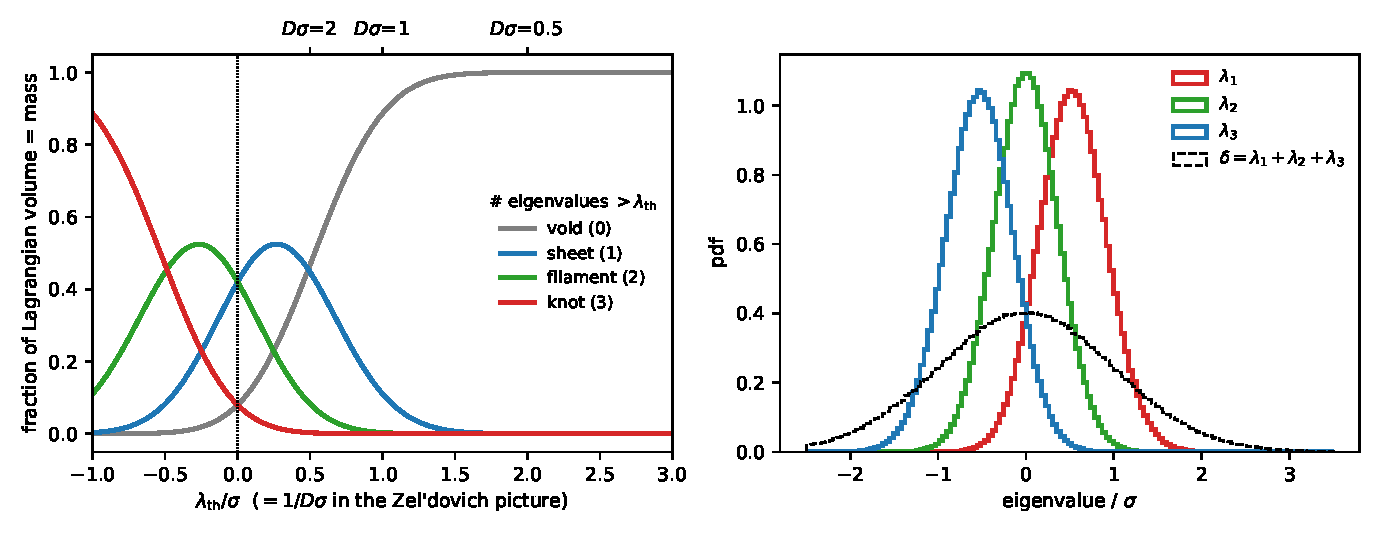
\includegraphics[width=0.85\textwidth]{figs/fig_web_stats.pdf}
\caption{\small סטטיסטיקה של רכיבי הרשת הקוסמית: צמתים, פילמנטים, לוחות וחללים, בנפח ובמסה.}
\end{figure}

% ---------------------------------------------------------------------
\subsection*{תרגילים}
\begin{exercise}{מסת ג'ינס לפני ואחרי הרקומבינציה}
ב-$z=1100$, עם $\Omega_mh^2=0.143$ ו-$\Omega_bh^2=0.0224$: (א) חשבו $\bar\rho_m$ ו-$\bar\rho_b$. (ב) לפני הרקומבינציה $c_s\simeq c/\sqrt{3(1+R)}$, $R\approx0.6$. חשבו $\lambda_J$ ומסת הבריונים $M_J$. (ג) אחרי הרקומבינציה גז מימן-הליום עם $T\approx3000\,\mathrm K$, $\mu=1.22$: $c_s=\sqrt{5k_BT/3\mu m_p}$. חשבו שוב. איזה עצם אסטרופיזיקלי יש לו מסה כזו?
\end{exercise}
\begin{solbox}
\textbf{פתרון.}\ (א) $1101^3=1.335\times10^9$: $\bar\rho_m=3.6\times10^{-18}$, $\bar\rho_b=5.6\times10^{-19}\,\mathrm{kg\,m^{-3}}$.\\
(ב) $c_s=c/\sqrt{4.8}=1.37\times10^5\,\kms$. $\lambda_J=c_s\sqrt{\pi/G\bar\rho_m}\approx0.5\,\Mpc$ פיזיקלי ($\approx560\,\Mpc$ נע). $M_J=\tfrac{4\pi}{3}\bar\rho_b(\lambda_J/2)^3\approx6\times10^{17}\Msun$: יותר מכל צביר. אין צמיחה בריונית.\\
(ג) $c_s=\sqrt{5k_BT/3\mu m_p}=5.8\,\kms$, $\lambda_J\approx22\,\mathrm{pc}$, $M_J\approx4\times10^4\Msun$: מסה של צביר כדורי. ירידה בפקטור $10^{13}$ בבת אחת.
\end{solbox}

\begin{exercise}{פתרונות הצמיחה}
(א) הראו ש-$\delta\propto t^{2/3}$ ו-$t^{-1}$ פותרים את \eqref{eq:growth} ב-\en{EdS} עם $c_s=0$. (ב) הראו שבמשתנה $\ln a$ המשוואה היא $\delta''+\tfrac12\delta'-\tfrac32\delta=0$. (ג) ביקום של $\Lambda$ בלבד ($H=$ קבוע, $\bar\rho_m\to0$), פתרו והראו ש-$\delta\to$ קבוע. מה זה אומר על מבנה בעתיד?
\end{exercise}
\begin{solbox}
\textbf{פתרון.}\ (א) $\delta=t^n$: $n(n-1)+\tfrac43n-\tfrac23=0\Rightarrow3n^2+n-2=0\Rightarrow n=\tfrac23,\,-1$.\\
(ב) $\frac{d}{dt}=H\frac{d}{d\ln a}$, $\ddot\delta=H^2\delta''+\dot H\delta'$, $\dot H=-\tfrac32H^2$: $H^2(\delta''+\tfrac12\delta')=\tfrac32H^2\delta$. פתרונות $a^1$, $a^{-3/2}$.\\
(ג) $\ddot\delta+2H\dot\delta=0$: $\delta=C_1+C_2e^{-2Ht}\to C_1$. המבנה "קופא": לא ייווצרו צבירים חדשים גדולים יותר.
\end{solbox}

\begin{exercise}{מאיפה $18\pi^2$?}
קליפה כדורית: $R=A(1-\cos\theta)$, $t=B(\theta-\sin\theta)$, עם $A^3=GMB^2$. (א) הראו שב-\en{turnaround} ($\theta=\pi$) הניגוד ביחס לרקע \en{EdS} הוא $1+\delta=9\pi^2/16\approx5.55$. (ב) משפט הוויריאל ושימור אנרגיה נותנים $R_{\rm vir}=R_{\rm ta}/2$, והקריסה ב-$t_{\rm coll}=2t_{\rm ta}$. הראו ש-$\Delta_{\rm vir}=18\pi^2\approx178$.
\end{exercise}
\begin{solbox}
\textbf{פתרון.}\ (א) ב-$\theta=\pi$: $R=2A$, $t=\pi B$. $\rho_{\rm sh}=3M/(32\pi A^3)$, $\bar\rho=1/(6\pi Gt^2)=1/(6\pi^3GB^2)$. היחס: $\frac{18\pi^2GMB^2}{32A^3}=\frac{9\pi^2}{16}$.\\
(ב) ב-$t=2\pi B$ ו-$R=A$: $\rho_{\rm vir}/\bar\rho=\frac{3M}{4\pi A^3}\cdot6\pi G(2\pi B)^2=18\pi^2=178$. (הדרך: $5.55\times2^3\times2^2$; $2^3$ מחצי הרדיוס, $2^2$ מהרקע שדולל בזמן כפול.)
\end{solbox}

% =====================================================================
\lecture{4}{עדויות לחומר אפל: ויריאל, קריסה כדורית, עקומות סיבוב, \en{NFW} ו-\en{MOND}}{מפגש 2, שעה. \ (10' ויריאל, 15' קריסה כדורית, 20' עקומות סיבוב ופרופילים, 10' התאמה, 5' \en{MOND}, תרגילים)}
% =====================================================================

\begin{goalbox}
\textbf{מטרות.} (1) להעריך מסה ממהירויות: משפט הוויריאל. (2) לגזור את מודל הקריסה הכדורית ($\delta_c$, $18\pi^2$, $r_{\rm vir}$) ולהשתמש בו כעדות לחומר אפל (טיעון התזמון). (3) לקרוא עקומת סיבוב ולהסיק ממנה פרופיל צפיפות. (4) להכיר את פרופיל \en{NFW} ולהתאים אותו לנתונים (אותה מכונה של הרצאה 2). (5) לדעת מה \en{MOND} מסביר ומה לא.
\end{goalbox}

\subsection{משפט הוויריאל: צבירי גלקסיות}
למערכת כבולה במצב יציב, ממוצע בזמן של $\frac{d^2I}{dt^2}=0$ ($I=\sum m r^2$):
\begin{equation}
2K+W=0 .
\end{equation}
לכדור אחיד: $W=-\frac35\frac{GM^2}{R}$; ומהירות נמדדת רק לאורך קו הראייה, $K=\frac12M\langle v^2\rangle=\frac32M\sigma_{\rm los}^2$. לכן
\begin{equation}
\boxed{\;M\simeq\frac{5\,\sigma_{\rm los}^2R}{G}\;}
\end{equation}
\textbf{\en{Zwicky} (1933), צביר \en{Coma}:} $\sigma\approx1000\,\kms$, $R\approx1.5\,\Mpc$ נותנים $M\sim2\times10^{15}\Msun$ ויחס מסה-אור $M/L\sim300$ (בשמש: 1, בכוכבים: $\sim3$). היום: גז חם בקרני \en{X} ועדשות כבידה נותנים אותה תמונה. בריונים (בעיקר גז) הם $\sim15\%$ מהמסה, כמו $\Omega_b/\Omega_m$ הקוסמי.

\subsection{קריסה כדורית: איך נוצרת הילה כבולה}\label{sec:sc}
\en{Zwicky} הניח שהצביר בשיווי משקל ויריאלי. מודל הקריסה הכדורית (\en{Gunn \& Gott 1972}) מסביר למה, באיזו צפיפות, ובאיזה רדיוס. הוא גם נותן שני מבחנים לחומר אפל שאינם תלויים בשיווי משקל: מסת החבורה המקומית מהדינמיקה שלה בלבד, וגודל ההילה סביב גלקסיה, שאותו בודקות עקומות הסיבוב (סעיף הבא).

\textbf{משוואת הקליפה.} כדור שצפיפותו מעט גבוהה מהרקע. לפי משפט \en{Birkhoff}, קליפה ברדיוס $R(t)$ מרגישה רק את המסה $M$ שבתוכה (כל עוד הקליפות אינן חוצות זו את זו):
\begin{equation}
\ddot R=-\frac{GM}{R^2}+\frac{\Lambda}{3}R,\qquad
\frac12\dot R^2-\frac{GM}{R}-\frac{\Lambda}{6}R^2=E .
\label{eq:sc-eom}
\end{equation}
הילות נוצרות בעיקר בעידן החומר, ולכן נתחיל ב-$\Lambda=0$ ורקע \en{EdS}. עם $E<0$ הקליפה קשורה: זהו יקום פרידמן קטן עם $k=+1$ (הרצאה 1).

\textbf{הפתרון (ציקלואידה).}
\begin{equation}
\boxed{\;R=A(1-\cos\theta),\qquad t=B(\theta-\sin\theta),\qquad A^3=GMB^2\;}
\label{eq:sc-cycloid}
\end{equation}
בדיקה: $\dot R=\frac{dR/d\theta}{dt/d\theta}=\frac{A}{B}\frac{\sin\theta}{1-\cos\theta}$. עם $\sin^2\theta=(1-\cos\theta)(1+\cos\theta)$ ו-$GM=A^3/B^2$:
\begin{equation}
E=\frac{A^2}{B^2}\Big[\frac{1+\cos\theta}{2(1-\cos\theta)}-\frac{1}{1-\cos\theta}\Big]=-\frac{A^2}{2B^2},
\end{equation}
קבוע ושלילי, כנדרש.
\begin{center}\small
\begin{tabular}{@{}cccl@{}}
\toprule
$\theta$ & $R$ & $t$ & משמעות \\ \midrule
$0$ & $0$ & $0$ & ההפרעה מתחילה עם הרקע \\
$\pi$ & $R_{\rm ta}=2A$ & $t_{\rm ta}=\pi B$ & נקודת המפנה (\en{turnaround}), $\dot R=0$ \\
$2\pi$ & $0$ & $t_{\rm coll}=2t_{\rm ta}$ & קריסה (פורמלית) \\ \bottomrule
\end{tabular}
\end{center}

\textbf{הניגוד בצפיפות.} $\rho_{\rm sh}=3M/4\pi R^3$ ו-$\bar\rho=1/6\pi Gt^2$ (\en{EdS}). היחס, אחרי שימוש ב-$A^3=GMB^2$:
\begin{equation}
1+\delta(\theta)=\frac92\,\frac{(\theta-\sin\theta)^2}{(1-\cos\theta)^3}.
\label{eq:sc-dNL}
\end{equation}
התוצאה אינה תלויה ב-$M$: כל ההפרעות הכדוריות עוברות אותו מסלול, כל אחת בקצב שלה.

\textbf{הגבול הלינארי.} ל-$\theta\ll1$: $\theta-\sin\theta\simeq\frac{\theta^3}{6}(1-\frac{\theta^2}{20})$, $1-\cos\theta\simeq\frac{\theta^2}{2}(1-\frac{\theta^2}{12})$, ולכן $\delta\simeq\frac{3}{20}\theta^2$. עם $t\simeq B\theta^3/6$:
\begin{equation}
\delta_L(t)=\frac{3}{20}\Big(\frac{6t}{B}\Big)^{2/3}\propto a ,
\end{equation}
המוד הגדל של הרצאה 3. $\delta_L$ הוא מה שהתורה הלינארית \emph{הייתה} נותנת; את השדה הלינארי קל לחשב, ולכן הוא משמש כשעון. בשתי נקודות:
\begin{center}\small
\begin{tabular}{@{}lcc@{}}
\toprule
 & $\delta$ אמיתי & $\delta_L$ \\ \midrule
מפנה, $\theta=\pi$ & $\frac{9\pi^2}{16}-1=4.55$ & $\frac{3}{20}(6\pi)^{2/3}=1.06$ \\
קריסה, $\theta=2\pi$ & $\infty$ & $\boxed{\delta_c=\frac{3}{20}(12\pi)^{2/3}=1.686}$ \\ \bottomrule
\end{tabular}
\end{center}
הילה נוצרת היכן שהשדה הלינארי, מוחלק בסולם $R(M)$, חוצה את $\delta_c$. זה הבסיס של \en{Press--Schechter} ופונקציות המסה של הילות.

\textbf{ויריאליזציה: $18\pi^2$.} קריסה לנקודה היא תוצר של סימטריה מושלמת. בפועל תנועה רדיאלית הופכת לתנועה אקראית והמערכת מתייצבת. משפט הוויריאל $2K+W=0$ נותן $E=W/2$. במפנה $K=0$, ולכן $E=W_{\rm ta}$. מאחר ש-$W\propto-1/R$:
\begin{equation}
\frac{W_{\rm vir}}{2}=W_{\rm ta}\ \Longrightarrow\ \boxed{R_{\rm vir}=\tfrac12R_{\rm ta}} .
\end{equation}
המקדם ש-$W$ תלוי בו (פרופיל הצפיפות) מתבטל. הניגוד הסופי, ב-$t_{\rm coll}=2t_{\rm ta}$:
\begin{equation}
\Delta_{\rm vir}\equiv\frac{\rho_{\rm vir}}{\bar\rho(t_{\rm coll})}
=\underbrace{\frac{9\pi^2}{16}}_{\rm turnaround}\times\underbrace{2^3}_{R\to R/2}\times\underbrace{2^2}_{\bar\rho\propto t^{-2}}=18\pi^2\approx178 .
\end{equation}
מכאן הגדרת ההילה: המסה בתוך $r_{\rm vir}$, שבו הצפיפות הממוצעת היא $\Delta$ פעמים צפיפות הייחוס,
\begin{equation}
M_{\rm vir}=\frac{4\pi}{3}\Delta\,\rho_{\rm ref}\,r_{\rm vir}^3,\qquad V_{\rm vir}^2=\frac{GM_{\rm vir}}{r_{\rm vir}} .
\label{eq:sc-rvir}
\end{equation}

\textbf{עם $\Lambda$.} שלושה שינויים:
\begin{itemize}
\item $\delta_c$ כמעט לא משתנה: $\approx1.68$ ב-$\LCDM$ (תלות חלשה ב-$\Omega_m$).
\item $\Delta$ משתנה. התאמה נומרית ביחס לצפיפות הקריטית (\en{Bryan \& Norman 1998}): $\Delta_c=18\pi^2+82x-39x^2$, $x=\Omega_m(z)-1$. היום $\Delta_c\approx103$, כלומר $\approx330\bar\rho_m$. המוסכמה $M_{200}$ ($200\rho_c$) היא עיגול של אותו רעיון.
\item משפט הוויריאל מקבל איבר של $\Lambda$. לכדור אחיד $W_\Lambda=-\frac{\Lambda}{10}MR^2$, ומ-$2K=-W_G+2W_\Lambda$ (לאיבר $\propto R^n$, $2K=nW$) מתקבל $2K+W_G=2W_\Lambda$ (\en{Lahav et al.\ 1991}; להכללה לאנרגיה אפלה דינמית: \en{Naderi, Malekjani \& Pace 2015}). שימור אנרגיה בין המפנה לוויריאל נותן, עם $y=R_{\rm vir}/R_{\rm ta}$ ו-$Q=\rho_\Lambda/\rho_{\rm ta}$:
\begin{equation}
4Qy^3-2(1+Q)y+1=0,\qquad y\simeq\tfrac12-\tfrac{Q}{4}.
\end{equation}
$\Lambda$ דוחה, ולכן ההילה קורסת לרדיוס קטן יותר. ומ-\eqref{eq:sc-eom}: קליפה נעצרת רק אם $\ddot R<0$ במפנה, כלומר $R_{\rm ta}<(3GM/\Lambda)^{1/3}$, רדיוס מפנה מקסימלי ($1.1\,\Mpc$ ל-$10^{12}\Msun$, $11\,\Mpc$ ל-$10^{15}\Msun$; \en{Pavlidou \& Tomaras 2014}).
\end{itemize}

\begin{keybox}
\textbf{למה זו עדות לחומר אפל.}
\begin{enumerate}
\item \textbf{טיעון התזמון} (\en{Kahn \& Woltjer 1959}). שביל החלב ו-\en{M31} נמצאים ב-$r\approx0.78\,\Mpc$ ומתקרבים ב-$v_r\approx-110\,\kms$. אם נפרדו במפץ ונעים במסלול רדיאלי, הם על הציקלואידה \eqref{eq:sc-cycloid} עם $t=t_0$:
\begin{equation}
\frac{v\,t_0}{r}=\frac{\sin\theta\,(\theta-\sin\theta)}{(1-\cos\theta)^2}=-1.99
\ \Rightarrow\ \theta=4.20,\quad M=\frac{A^3}{GB^2}\approx4\times10^{12}\Msun
\end{equation}
(תרגיל 4.4). עם $\Lambda$ וכיול על סימולציות: $\sim5\times10^{12}\Msun$ (\en{Li \& White 2008}). הכוכבים והגז בשתי הגלקסיות: $\sim2\times10^{11}\Msun$. חסר פקטור $\sim20$. החישוב משתמש רק בכבידה ובגיל היקום, בלי הנחה על שיווי משקל.
\item \textbf{גודל ההילה.} הילה של $10^{12}\Msun$ היום: מ-\eqref{eq:sc-rvir} עם $\Delta_c=103$, $r_{\rm vir}\approx260\,\kpc$ ו-$V_{\rm vir}\approx130\,\kms$. הדיסקה הכוכבית נגמרת ב-$\sim15$--$20\,\kpc$. החיזוי: מסה שמשתרעת פי $\sim10$ מעבר לאור, ומהירויות סיבוב של $\sim100$--$200\,\kms$ הרחק מהדיסקה (הריכוז, סעיף~\ref{sec:nfw}, מעלה את $v_c$ בפנים). זה בדיוק מה שעקומות הסיבוב בודקות.
\item \textbf{מתי.} הילה נוצרת כש-$\delta_L$ מגיע ל-$1.686$. בריונים לבדם מגיעים היום ל-$\delta_L\sim10^{-2}$ (הרצאה 3), כלומר לא הייתה נוצרת אף הילה. עם \en{CDM}, הילות בגודל גלקסיה קורסות ב-$z\sim1$--$3$.
\end{enumerate}
\end{keybox}

\subsection{עקומות סיבוב}
למסלול מעגלי בפוטנציאל כדורי:
\begin{equation}
v_c^2(r)=\frac{GM(<r)}{r}.
\end{equation}
\begin{itemize}
\item מחוץ לרוב המסה הנראית: $v_c\propto r^{-1/2}$ (קפלר).
\item נצפה (\en{Rubin}, קווי \en{HI} באורך 21 ס"מ, 1970--80): $v_c\approx$ קבוע עד רדיוסים גדולים בהרבה מהדיסקה.
\item $v_c=$ קבוע $\Rightarrow M(<r)\propto r\Rightarrow\rho\propto r^{-2}$: \textbf{הילה איזותרמית}.
\end{itemize}
המהירות הכוללת היא סכום ריבועים של הרכיבים (פואסון לינארי):
\begin{equation}
v_c^2=\Upsilon_\star v_\star^2+v_{\rm gas}^2+v_{\rm DM}^2,
\end{equation}
עם $\Upsilon_\star$ יחס מסה-אור של הכוכבים. לדיסקה אקספוננציאלית ($\Sigma\propto e^{-R/R_d}$) $v_\star$ מגיעה לשיא ב-$2.2R_d$ ויורדת.

\subsection{פרופילי הילה}\label{sec:nfw}
\begin{keybox}
\textbf{\en{NFW}} (\en{Navarro, Frenk \& White 1997}) --- פרופיל אוניברסלי של הילות בסימולציות \en{CDM}:
\begin{equation}
\rho(r)=\frac{\rho_s}{(r/r_s)(1+r/r_s)^2},\qquad
M(<r)=4\pi\rho_sr_s^3\Big[\ln(1+x)-\frac{x}{1+x}\Big],\ \ x=r/r_s .
\end{equation}
$\rho\propto r^{-1}$ במרכז (\textbf{קאספ}) ו-$r^{-3}$ בחוץ. המסה מתבדרת לוגריתמית, ולכן מגדירים $M_{200}$: המסה בתוך $r_{200}$ שבו הצפיפות הממוצעת $=200\rho_c$. פרמטר הריכוז $c=r_{200}/r_s\sim5$--$15$, ויורד לאט עם המסה. $v_c$ מקסימלית ב-$r=2.163\,r_s$.
\end{keybox}
\textbf{ליבות מול קאספים.} בגלקסיות ננס רבות הנתונים מעדיפים ליבה, $\rho\to$ קבוע: איזותרמית-מדומה $\rho_0/[1+(r/r_c)^2]$ או \en{Burkert} $\rho_0r_0^3/[(r+r_0)(r^2+r_0^2)]$. הסבר אפשרי: משוב מסופרנובות שמזיז גז ושוטח את המרכז. או חומר אפל שאינו קר לגמרי (\en{SIDM}, \en{fuzzy DM}).

\subsection{התאמת פרופיל לעקומת סיבוב}
אותה מכונה של הרצאה 2:
\begin{enumerate}
\item נתונים: $(r_i,v_i,\sigma_i)$; רכיבים בריוניים $v_\star(r),v_{\rm gas}(r)$ מפוטומטריה ומ-\en{HI}.
\item מודל: $v^2=\Upsilon_\star v_\star^2+v_{\rm gas}^2+v_{\rm NFW}^2(r;M_{200},c)$.
\item $\chi^2=\sum_i(v_i-v(r_i))^2/\sigma_i^2$; מוקדמות: $\Upsilon_\star$ מאוכלוסיות כוכבים, יחס $c(M)$ מסימולציות.
\item \en{MCMC} על $(\log M_{200},c,\Upsilon_\star)$ ו-\en{corner}.
\end{enumerate}
\textbf{ניוון דיסקה-הילה:} דיסקה כבדה יותר ($\Upsilon_\star$ גדול) מפוצה בהילה עם ריכוז נמוך. זו אותה בננה שראינו ב-$(\Omega_m,w)$. ההנחה "דיסקה מקסימלית" היא הגבול העליון של הניוון.

\begin{figure}[htbp]\centering
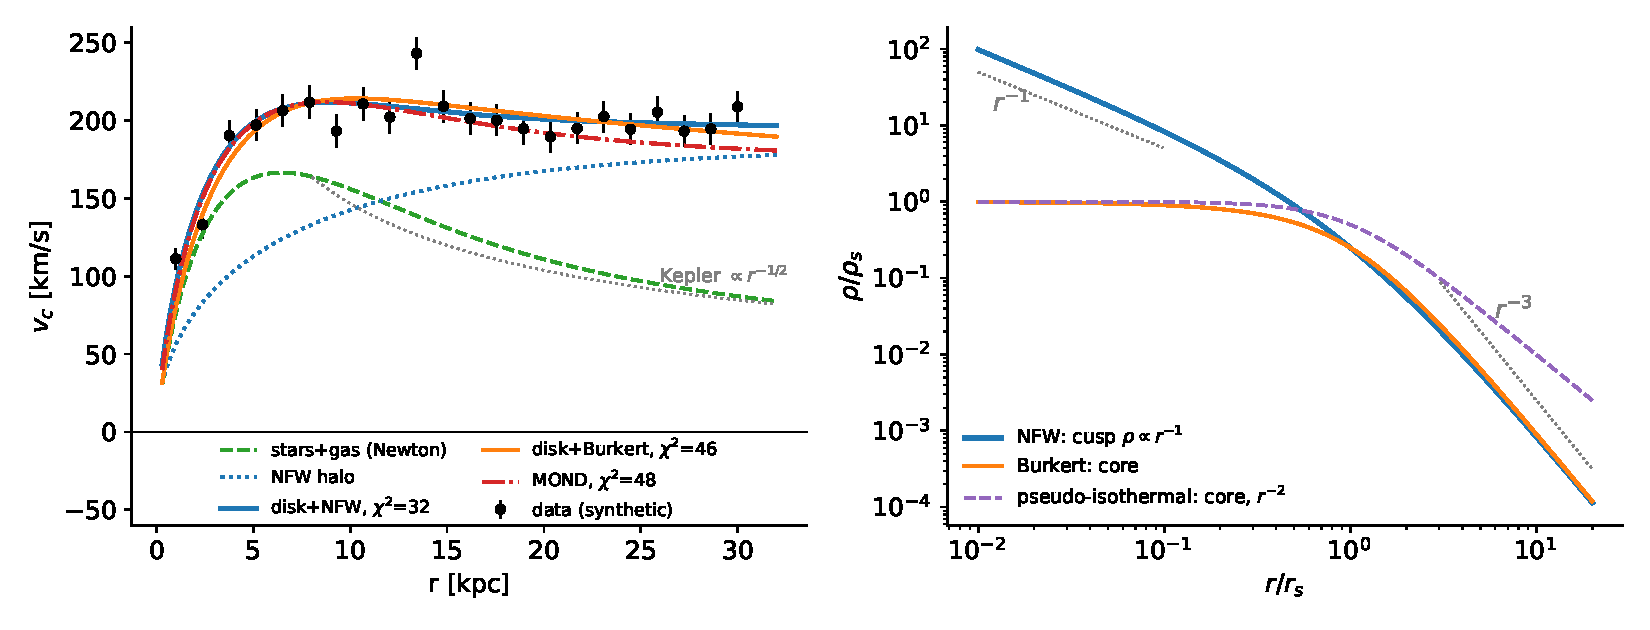
\includegraphics[width=\textwidth]{figs/fig_rotcurve_nfw.pdf}
\caption{\small שמאל: עקומת סיבוב סינתטית (נוצרה מ-\en{NFW}), מותאמת בדיסקה+\en{NFW}, דיסקה+\en{Burkert}, ו-\en{MOND} ללא חומר אפל. הכוכבים לבדם (ירוק) יורדים כמו קפלר; הנתונים לא. ימין: צורת הפרופילים --- קאספ מול ליבה. הסקריפט: \en{scripts/make\_new\_figs.py}.}
\end{figure}

\subsection{עדויות נוספות (בקצרה)}
עדשות כבידה חזקות וחלשות ממפות מסה ישירות; \en{Bullet Cluster}: מרכז המסה (עדשות) נפרד מהגז החם (קרני \en{X}) אחרי התנגשות; ה-\en{CMB}: יחס גובה הפסגות האי-זוגיות לזוגיות דורש $\Omega_ch^2\approx0.12$ (הרצאה 5); וצמיחת מבנה (הרצאה 3).

\subsection{\en{MOND} --- בקצרה}
\en{Milgrom} (1983): לא חומר חסר אלא דינמיקה שונה בתאוצות נמוכות.
\begin{equation}
\mu\!\Big(\frac{g}{a_0}\Big)\,g=g_N,\qquad a_0\approx1.2\times10^{-10}\,\mathrm{m\,s^{-2}},\qquad \mu(x)\to\begin{cases}1&x\gg1\\x&x\ll1\end{cases}
\end{equation}
בגבול העמוק $g=\sqrt{g_Na_0}$, ומ-$v^2/r=\sqrt{GMa_0}/r$:
\begin{equation}
v_{\rm flat}^4=GM_ba_0 \qquad(\text{\en{baryonic Tully--Fisher}}).
\end{equation}
\begin{center}\small
\begin{tabular}{@{}p{7cm}p{7cm}@{}}
\toprule
\textbf{הצלחות} & \textbf{קשיים} \\ \midrule
עקומות סיבוב של גלקסיות עם פרמטר אחד ($a_0$) & צבירים: עדיין חסר פקטור $\sim2$ במסה \\
יחס \en{Tully--Fisher} הבריוני, כולל השיפוע 4 & \en{Bullet Cluster}: המסה לא עוקבת אחרי הבריונים \\
הקשר ההדוק $g_{\rm obs}(g_{\rm bar})$ (\en{RAR}) & ה-\en{CMB} וספקטרום ההספק: ללא רכיב לא-בריוני --- פסגה שלישית נמוכה מדי \\
& אין תיאוריה יחסותית פשוטה ומקובלת (\en{TeVeS} נפסלה עם \en{GW170817}) \\ \bottomrule
\end{tabular}
\end{center}
המסקנה המקובלת: \en{MOND} הוא תיאור מוצלח של \emph{גלקסיות}, וכל מודל חומר אפל חייב לשחזר את ה-\en{RAR}; בסולמות קוסמולוגיים \en{CDM} עדיף בבירור.

% ---------------------------------------------------------------------
\subsection*{תרגילים}
\begin{exercise}{\en{Zwicky} ו-\en{Coma}}
(א) גזרו $M=5\sigma_{\rm los}^2R/G$ ממשפט הוויריאל לכדור אחיד. (ב) עם $\sigma_{\rm los}=1000\,\kms$, $R=1.5\,\Mpc$ ו-$L\approx5\times10^{12}L_\odot$ חשבו $M$ ו-$M/L$. (ג) זמן החצייה $R/\sigma$ --- האם הוא קצר מגיל היקום? למה זה חשוב לשימוש בוויריאל?
\end{exercise}
\begin{solbox}
\textbf{פתרון.}\ (א) $2K+W=0$, $K=\tfrac32M\sigma^2$, $W=-\tfrac35GM^2/R\Rightarrow M=5\sigma^2R/G$.\\
(ב) $M=5(10^6)^2(4.6\times10^{22})/6.67\times10^{-11}=3.5\times10^{45}\,\mathrm{kg}=1.7\times10^{15}\Msun$. $M/L\approx350$.\\
(ג) $R/\sigma=1.5\,\Gyr\ll t_0$: הצביר עבר כמה זמני חצייה, ולכן סביר שהוא קרוב לשיווי משקל ויריאלי.
\end{solbox}

\begin{exercise}{פרופיל \en{NFW}}
(א) גזרו את $M(<r)$ מ-$\rho_{\rm NFW}$. (ב) מצאו את האסימפטוטות של $v_c(r)$ ב-$r\ll r_s$ וב-$r\gg r_s$. (ג) הראו ש-$v_c$ מקסימלית כאשר $\ln(1+x)=\frac{x(2x+1)}{(1+x)^2}$, ופתרו נומרית ($x\approx2.16$). (ד) לגלקסיה עם $v_{\max}=200\,\kms$ ב-$r_{\max}=40\,\kpc$, מצאו $r_s$ ו-$\rho_s$.
\end{exercise}
\begin{solbox}
\textbf{פתרון.}\ (א) $M=4\pi\rho_sr_s^3\int_0^x\frac{x'\,dx'}{(1+x')^2}=4\pi\rho_sr_s^3[\ln(1+x)-\frac{x}{1+x}]$.\\
(ב) $x\ll1$: $M\approx2\pi\rho_sr_s^3x^2$, $v\propto r^{1/2}$. $x\gg1$: $M\propto\ln x$, $v^2\propto\ln r/r$ (יורד לאט).\\
(ג) $\frac{d}{dx}[m(x)/x]=0\Rightarrow xm'=m$, $m'=x/(1+x)^2$. מכאן $\ln(1+x)=\frac{x}{1+x}+\frac{x^2}{(1+x)^2}=\frac{x(2x+1)}{(1+x)^2}$; $x=2.163$, $m(x)/x=0.2162$.\\
(ד) $r_s=40/2.163=18.5\,\kpc$. $v_{\max}^2=4\pi G\rho_sr_s^2\times0.2162\Rightarrow\rho_s=1.0\times10^7\Msun\,\kpc^{-3}$.
\end{solbox}

\begin{exercise}{\en{MOND} בגלקסיה אחת}
גלקסיה עם $M_b=6\times10^{10}\Msun$. (א) באיזה רדיוס $r_M$ התאוצה הניוטונית משתווה ל-$a_0$? (ב) מה $v_{\rm flat}$ שחוזה \en{MOND}? (ג) ב-$r=30\,\kpc$ (נקודה מסה): חשבו $v$ ניוטוני ו-$v$ של \en{MOND} עם $\mu(x)=x/(1+x)$. (ד) גלקסיה עם מסה בריונית גדולה פי 16: פי כמה $v_{\rm flat}$?
\end{exercise}
\begin{solbox}
\textbf{פתרון.}\ (א) $r_M=\sqrt{GM_b/a_0}=8.3\,\kpc$.\\
(ב) $v_{\rm flat}=(GM_ba_0)^{1/4}=176\,\kms$.\\
(ג) $v_N=\sqrt{GM/r}=93\,\kms$. $g=\tfrac12g_N+\sqrt{g_N^2/4+g_Na_0}$ עם $g_N=9.3\times10^{-12}\,\mathrm{m\,s^{-2}}$: $g=3.8\times10^{-11}$, $v=188\,\kms$ (ושואף ל-176 ברדיוס גדול). כמו שחומר אפל היה נותן.\\
(ד) $16^{1/4}=2$. ב-\en{CDM} היחס הזה אינו נובע אוטומטית; הוא דורש שהבריונים יעקבו אחרי ההילה.
\end{solbox}

\begin{exercise}{טיעון התזמון של החבורה המקומית}
(א) מהציקלואידה \eqref{eq:sc-cycloid} הראו ש-$\frac{vt}{r}=\frac{\sin\theta(\theta-\sin\theta)}{(1-\cos\theta)^2}$. (ב) עם $r=0.78\,\Mpc$, $v=-110\,\kms$ ו-$t_0=13.8\,\Gyr$, פתרו נומרית ל-$\theta$ (רמז: הזוג כבר אחרי המפנה, $\pi<\theta<2\pi$) ומצאו $A$, $B$ ו-$M$. (ג) מה היה המרחק המקסימלי ומתי? (ד) השוו למסה הבריונית $\sim2\times10^{11}\Msun$. (ה) איך ישתנה $M$ אם $|v|$ גדל ב-10\%?
\end{exercise}
\begin{solbox}
\textbf{פתרון.}\ (א) $v=\dot R=\frac AB\frac{\sin\theta}{1-\cos\theta}$, $t/r=\frac{B(\theta-\sin\theta)}{A(1-\cos\theta)}$; המכפלה נותנת את הביטוי.\\
(ב) ביחידות $1\,\Mpc/\kms=977.8\,\Gyr$: $t_0=0.01411\,\Mpc/\kms$, ולכן $vt_0/r=-110\times0.01411/0.78=-1.99$. פתרון: $\theta=4.20$. $A=r/(1-\cos\theta)=0.523\,\Mpc$, $B=t_0/(\theta-\sin\theta)=2.72\,\Gyr$. $M=A^3/GB^2=4.3\times10^{12}\Msun$ (עם $G=4.30\times10^{-9}\,\Mpc\,(\kms)^2/\Msun$).\\
(ג) $R_{\max}=2A=1.05\,\Mpc$ ב-$t_{\rm ta}=\pi B=8.5\,\Gyr$, לפני כ-5 מיליארד שנה.\\
(ד) $M/M_b\approx20$: רוב המסה של החבורה המקומית אינה בכוכבים ובגז.\\
(ה) $|v|=121\,\kms$: $M\approx4.8\times10^{12}\Msun$, עלייה של $\sim11\%$. התוצאה חסינה יחסית לשגיאות במהירות.
\end{solbox}

% =====================================================================
\lecture{5}{היקום החם, הסקאלה האקוסטית ו-\en{BAO}}{מפגש 3, שעה וחצי. \ (20' היסטוריה תרמית ורקומבינציה, 30' גלי קול ואופק הקול, 20' \en{BAO}, 20' \en{DESI} והמתחים + תרגילים)}
% =====================================================================

\begin{goalbox}
\textbf{מטרות.} (1) להבין מתי ולמה היקום נעשה שקוף. (2) לחשב את אופק הקול $r_s$ ואת הזווית $\theta_\star$ של הפסגה האקוסטית. (3) לראות שאותו סרגל מופיע בהתפלגות הגלקסיות (\en{BAO}), ומה \en{DESI} מודד. (4) להכיר את המתחים היום: $H_0$, $\Omega_m$ ו-$w_0w_a$.
\end{goalbox}

\subsection{היסטוריה תרמית}
$T=T_0(1+z)$, $T_0=2.7255\,\mathrm K$. כלל אחד: תהליך בשיווי משקל כל עוד קצבו $\Gamma\gg H$; כש-$\Gamma\lesssim H$ הוא "קופא".
\begin{center}\small
\begin{tabular}{@{}llll@{}}
\toprule
אירוע & $T$ & $z$ & מה קורה \\ \midrule
התנתקות נייטרינו & $1\,\mathrm{MeV}$ & $10^{10}$ & $\Gamma_{\rm weak}\sim G_F^2T^5<H$ \\
\en{BBN} & $0.1\,\mathrm{MeV}$ & $4\times10^8$ & $Y_p\approx0.25$, דאוטריום $\Rightarrow\Omega_bh^2$ \\
שוויון קרינה-חומר & $0.8\,\mathrm{eV}$ & $3400$ & סוף שליטת הקרינה \\
רקומבינציה / פיזור אחרון & $0.26\,\mathrm{eV}$ & $1090$ & $e^-+p\to\mathrm H$; פוטונים חופשיים \\
\bottomrule
\end{tabular}
\end{center}
\textbf{למה $0.26\,\mathrm{eV}$ ולא $13.6\,\mathrm{eV}$?} על כל בריון יש $\eta^{-1}\approx1.6\times10^{9}$ פוטונים. גם כש-$T\ll13.6\,\mathrm{eV}$, הזנב של התפלגות פלאנק מכיל מספיק פוטונים מייננים. מימן נשאר מיונן עד $\eta^{-1}e^{-13.6\,\mathrm{eV}/T}\lesssim1$ (משוואת \en{Saha} מדייקת: $T\approx0.3\,\mathrm{eV}$).

\subsection{נוזל הפוטונים-בריונים וגלי קול}
לפני הרקומבינציה פיזור תומסון צמד בין הפוטונים לאלקטרונים, ואלה לפרוטונים: נוזל אחד. הלחץ מהפוטונים, האינרציה גם מהבריונים:
\begin{equation}
c_s=\frac{c}{\sqrt{3(1+R)}},\qquad R\equiv\frac{3\rho_b}{4\rho_\gamma}=\frac{3\Omega_b}{4\Omega_\gamma}\,\frac{1}{1+z}\approx0.6\ \text{ב-}z_\star .
\end{equation}
זו משוואה \eqref{eq:growth} של הרצאה 3 בגבול $k\gg k_J$: מתנד. בורות הפוטנציאל נוצרים מחומר אפל, והנוזל מתנודד בהם: דחיסה ונדירות.

\textbf{אופק הקול} --- המרחק הנע שגל קול עבר עד הרקומבינציה:
\begin{equation}
\boxed{\;r_s(z_\star)=\int_{z_\star}^{\infty}\frac{c_s(z)\,dz}{H(z)}\approx144\,\Mpc\;}
\qquad(\text{ובעידן הגרירה } z_d\approx1060:\ r_d\approx147\,\Mpc).
\end{equation}
$r_s$ תלוי רק בפיזיקה המוקדמת: $\Omega_bh^2$, $\Omega_mh^2$ ומספר הנייטרינו --- כולם ידועים מה-\en{CMB} עצמו. לכן זהו \textbf{סרגל תקני מכויל}.

\subsection{הפסגות האקוסטיות}
מוד $k$ נמצא בקיצון של התנודה ברגע הפיזור האחרון אם
\begin{equation}
k_n\,r_s=n\pi\qquad(n=1:\ \text{דחיסה ראשונה},\ n=2:\ \text{נדירות ראשונה},\dots)
\end{equation}
מוד $k$ נראה בשמיים בזווית $\theta\simeq\pi/(kD_M)$, ולכן $\ell\simeq kD_M(z_\star)$. הסקאלה האקוסטית:
\begin{equation}
\theta_\star=\frac{r_s(z_\star)}{D_M(z_\star)}=\frac{144}{13\,870}\approx0.0104\ \text{רד'}\ (0.6^\circ),\qquad
\ell_A=\frac{\pi}{\theta_\star}\approx302 .
\end{equation}
הפסגה הראשונה נמצאת ב-$\ell_1\approx220$, נמוך מ-$\ell_A$ בגלל היסט פאזה. \en{Planck} מודד את $\theta_\star$ לדיוק $0.03\%$ --- המספר המדויק ביותר בקוסמולוגיה.
\begin{itemize}
\item \textbf{עקמומיות:} $D_M(z_\star)$ תלוי ב-$\Omega_k$; $k>0$ מזיז את הפסגות לזוויות גדולות ($\ell$ קטן). התצפית: $\Omega_k\approx0$.
\item \textbf{בריונים:} $R$ מעמיק את הדחיסות $\Rightarrow$ פסגות אי-זוגיות גבוהות מזוגיות.
\item \textbf{חומר אפל:} גובה הפסגה השלישית $\Rightarrow\Omega_ch^2=0.120\pm0.001$.
\item \textbf{ריסון (\en{Silk damping}):} פוטונים מתפזרים לאורך $\sim10\,\Mpc$; פסגות ב-$\ell\gtrsim1000$ דועכות.
\end{itemize}

\begin{figure}[htbp]\centering
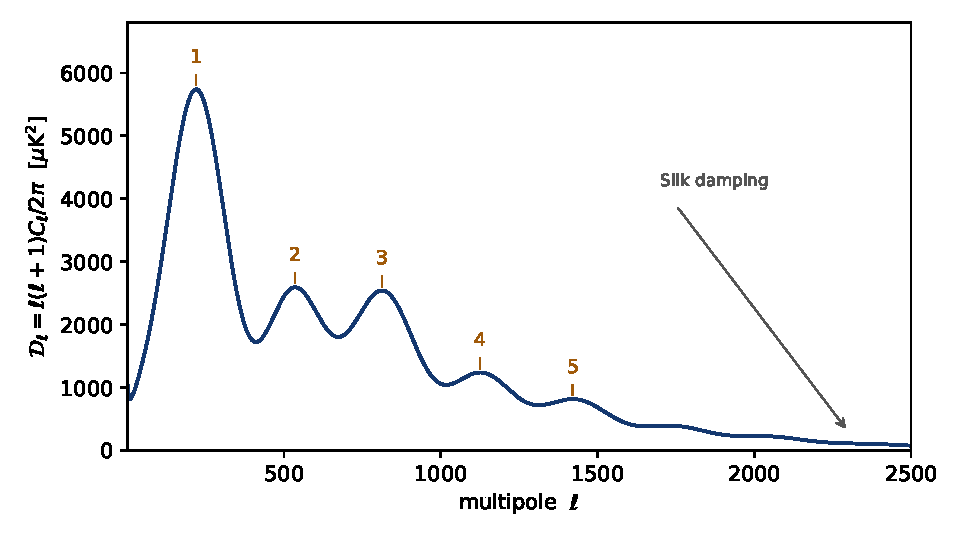
\includegraphics[width=0.49\textwidth]{figs/cmb_tt.pdf}\hfill
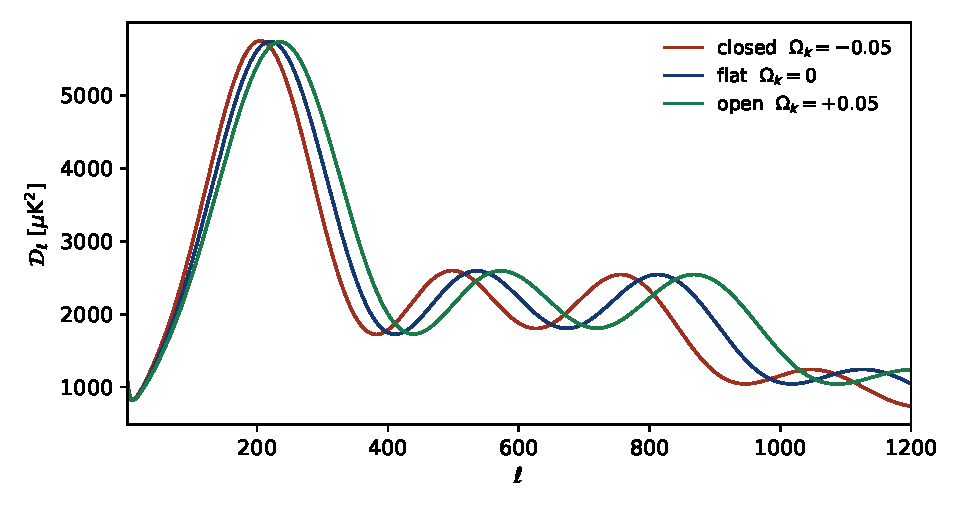
\includegraphics[width=0.49\textwidth]{figs/cmb_curvature.pdf}
\caption{\small שמאל: ספקטרום ה-\en{TT}, הפסגות האקוסטיות. ימין: הזזת הפסגה הראשונה עם העקמומיות.}
\end{figure}

\subsection{\en{BAO}: אותו סרגל בגלקסיות}
כל הפרעה התחילה כגל קול כדורי; בעידן הגרירה הגל "קפא" בבריונים במרחק $r_d$ מהמרכז, והחומר האפל נשאר במרכז. שניהם משכו זה את זה, ולכן בפונקציית המתאם של גלקסיות יש עודף במרחק נע $r_d\approx147\,\Mpc\approx100\,h^{-1}\Mpc$ (תנודות ב-$P(k)$).
\begin{equation}
\Delta\theta=\frac{r_d}{D_M(z)}\ \ (\text{רוחבי}),\qquad
\Delta z=\frac{r_d\,H(z)}{c}=\frac{r_d}{D_H(z)}\ \ (\text{לאורך קו הראייה}),\qquad
D_V=\big[z\,D_M^2D_H\big]^{1/3}.
\end{equation}
\begin{keybox}
\textbf{מה \en{BAO} מודד:} $D_M/r_d$ ו-$D_H/r_d$ כפונקציה של $z$. בלי ערך ל-$r_d$ מקבלים את $\Omega_m$ ואת $h\,r_d$ בלבד; עם $r_d$ מה-\en{CMB} או מ-\en{BBN} (עם $\Omega_bh^2$) מקבלים $H_0$. היחס $D_M/D_H$ (\en{Alcock--Paczynski}) לא תלוי ב-$r_d$ בכלל.
\end{keybox}

\begin{figure}[htbp]\centering
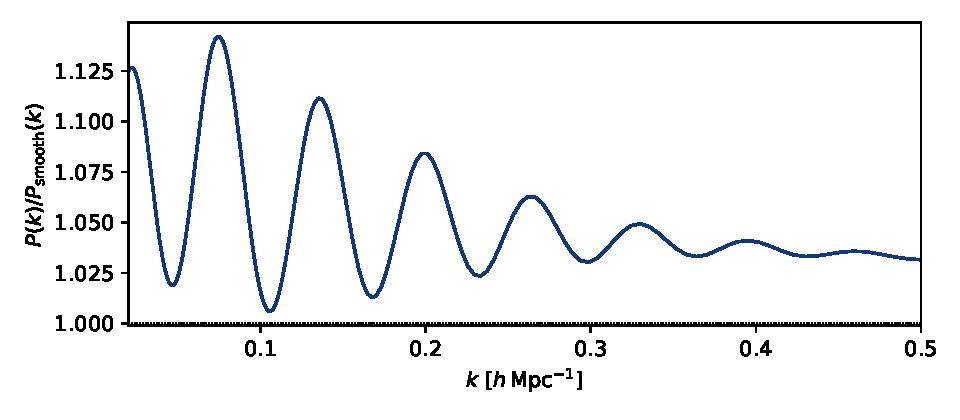
\includegraphics[width=0.55\textwidth]{figs/bao.pdf}
\caption{\small פיק ה-\en{BAO} בפונקציית המתאם, ב-$\approx100\,h^{-1}\Mpc$.}
\end{figure}

\subsection{\en{DESI DR2} והמתחים היום}
\en{DESI} (\en{Dark Energy Spectroscopic Instrument}; תוצאות \en{DR2} מתוך \en{arXiv:2503.14738}): $>14$ מיליון הסחות, שבע קבוצות עוקבים ב-$0.1<z<4.2$ (גלקסיות \en{BGS}, \en{LRG}, \en{ELG}, קוואזרים ויער \en{Ly$\alpha$}).
\begin{center}\small
\begin{tabular}{@{}p{5.6cm}p{1.4cm}p{8.8cm}@{}}
\toprule
צירוף נתונים & מודל & תוצאה \\ \midrule
\en{DESI} לבד & $\LCDM$ & $\Omega_m=0.2975\pm0.0086$, \ $h\,r_d=101.54\pm0.73\,\Mpc$ \\
\en{DESI+BBN} & $\LCDM$ & $H_0=68.51\pm0.58\,\kmsMpc$ \\
\en{DESI+CMB} & $w_0w_a$ & $w_0=-0.42\pm0.21$, $w_a=-1.75\pm0.58$; העדפה $3.1\sigma$ על $\Lambda$ \\
\en{DESI+CMB+SNe} & $w_0w_a$ & העדפה של \en{$2.8\sigma$ (Pantheon+), $3.8\sigma$ (Union3), $4.2\sigma$ (DESY5)} \\ \bottomrule
\end{tabular}
\end{center}

\begin{figure}[htbp]\centering
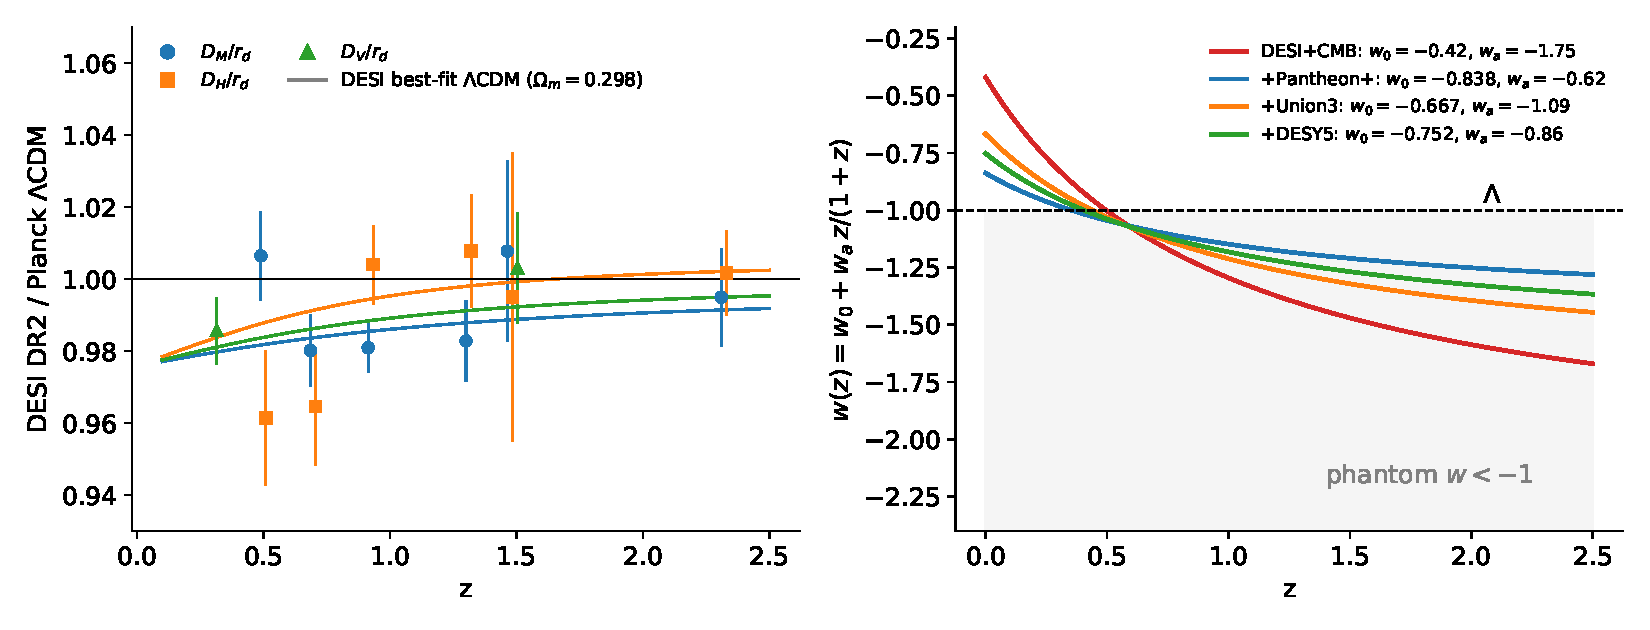
\includegraphics[width=\textwidth]{figs/fig_desi_bao.pdf}
\caption{\small שמאל: מרחקי \en{DESI DR2} ביחס ל-$\LCDM$ של \en{Planck}; הקו הרציף הוא ההתאמה הטובה ביותר של \en{DESI} ל-$\LCDM$ ($\Omega_m$ נמוך יותר). ימין: $w(z)$ של ארבע התאמות $w_0w_a$: כולן חוצות את $-1$ ליד $z\approx0.5$.}
\end{figure}

\textbf{שלושה מתחים, ומה לקחת מהם:}
\begin{enumerate}
\item \textbf{$H_0$.} סולם המרחקים (\en{SH0ES}, צפייניים${}+$\en{SNe}): $73.0\pm1.0$ (\en{Riess et al.\ 2022, ApJL 934, L7}). שיטות "הסרגל ההפוך" (\en{CMB}, או \en{BAO+BBN}): $67$--$68.5$. פער של $\sim4$--$5\sigma$. פתרון מוקדם חייב להקטין את $r_d$ בכ-$7\%$.
\item \textbf{$\Omega_m$.} \en{DESI} מעדיף $\Omega_m$ נמוך מעט מ-\en{Planck} ($0.315$); פער של $\sim2\sigma$ ב-$\LCDM$.
\item \textbf{אנרגיה אפלה דינמית.} $w_0>-1$, $w_a<0$: אנרגיה אפלה שהייתה "פנטום" ($w<-1$) בעבר ונחלשת היום. \emph{הסתייגויות:} תלוי בפרמטריזציה (\en{CPL}); תלוי בקטלוג הסופרנובות (טווח $2.8$--$4.2\sigma$); ומתקשר לגבול על מסת הנייטרינו ($\sum m_\nu<0.064\,\mathrm{eV}$ ב-$\LCDM$, לחץ לכיוון ערכים "שליליים").
\end{enumerate}
\textbf{קשר להרצאה 2:} אותה מכונה --- $\chi^2=\mathbf r^{\!\top}\mathsf C^{-1}\mathbf r$ בכל סל, עם מטריצה $2\times2$ ל-$(D_M/r_d,D_H/r_d)$. תרגיל הבית \en{HW 9B} בונה את כל הניתוח.

% ---------------------------------------------------------------------
\subsection*{תרגילים}
\begin{exercise}{מתי היקום נעשה שקוף?}
(א) הראו שמספר הפוטונים עם $E>13.6\,\mathrm{eV}$ לכל בריון הוא בערך $\eta^{-1}e^{-13.6\,\mathrm{eV}/k_BT}$ (עבור $k_BT\ll13.6\,\mathrm{eV}$, עד גורם פולינומי). (ב) עם $\eta=6\times10^{-10}$, מצאו את $T$ שבו המספר הזה הוא 1, ואת $z$ המתאים. (ג) \en{Saha} נותן $T\approx0.3\,\mathrm{eV}$. מה ההבדל בין רקומבינציה להתנתקות ($\Gamma_T=n_e\sigma_Tc=H$)?
\end{exercise}
\begin{solbox}
\textbf{פתרון.}\ (א) $n_\gamma(E>I)\propto\int_{I/T}^\infty x^2e^{-x}dx\approx(I/T)^2e^{-I/T}$; לבריון: $\eta^{-1}(I/T)^2e^{-I/T}$ עד קבוע $\sim0.4$.\\
(ב) $\eta^{-1}e^{-I/T}=1\Rightarrow T=I/\ln(1/\eta)=13.6/21.2=0.64\,\mathrm{eV}$, $z\approx2700$. הערכה גסה (הגורם הפולינומי מזיז את התשובה למטה).\\
(ג) רקומבינציה: $x_e$ יורד ל-$\sim0.5$ ב-$T\approx0.3\,\mathrm{eV}$ ($z\approx1300$). התנתקות: $n_e\sigma_Tc=H$, כש-$x_e\sim10^{-2}$, ב-$z\approx1090$. הפוטונים משתחררים מעט אחרי שהמימן נוצר.
\end{solbox}

\begin{exercise}{אופק הקול והפסגה הראשונה}
(א) בהזנחת $R$, ובחומר${}+$קרינה, הראו ש-
\[r_s=\frac{2c}{\sqrt3\,H_0\sqrt{\Omega_m}}\Big[\sqrt{a_\star+a_{\rm eq}}-\sqrt{a_{\rm eq}}\Big].\]
(ב) הציבו $\Omega_mh^2=0.143$, $z_\star=1090$, $z_{\rm eq}=3400$. כמה יוצא? מה יקרה כשמכניסים $R\approx0.6$? (התשובה המדויקת: $144\,\Mpc$.) (ג) עם $D_M(z_\star)=13.9\,\mathrm{Gpc}$, חשבו $\theta_\star$ ו-$\ell_A$. (ד) אם $\Omega_k=+0.05$, לאיזה כיוון זזה הפסגה?
\end{exercise}
\begin{solbox}
\textbf{פתרון.}\ (א) $r_s=\int c_s\,dt/a=\int c_s\,da/(a^2H)$ עם $a^2H=H_0\sqrt{\Omega_m}\sqrt{a+a_{\rm eq}}$; $\int_0^{a_\star}da/\sqrt{a+a_{\rm eq}}=2[\sqrt{a_\star+a_{\rm eq}}-\sqrt{a_{\rm eq}}]$.\\
(ב) $\frac{2c}{\sqrt3H_0\sqrt{\Omega_m}}=9150\,\Mpc$. בלי קרינה: $277\,\Mpc$; עם קרינה: $162\,\Mpc$; עם $R$ (מקטין את $c_s$ עד $\times0.79$ ב-$z_\star$): $144\,\Mpc$.\\
(ג) $\theta_\star=144/13\,900=0.0104$ רד' $=0.60^\circ$, $\ell_A=\pi/\theta_\star\approx302$ (הפסגה הראשונה ב-$\ell_1\approx220$ בגלל היסט פאזה).\\
(ד) $\Omega_k>0$ (סגור): $D_M$ קטן יותר, $\theta_\star$ גדול יותר, הפסגה זזה ל-$\ell$ נמוך יותר.
\end{solbox}

\begin{exercise}{נקודת \en{DESI} אחת}
\en{LRG2} ב-$z=0.706$: $D_M/r_d=17.35\pm0.18$, $D_H/r_d=19.46\pm0.33$. (א) עם $r_d=147.09\,\Mpc$, חשבו $D_M$ ו-$H(z)$. (ב) השוו ל-$\LCDM$ של \en{Planck} ($h=0.674$, $\Omega_m=0.315$). בכמה אחוזים ובכמה $\sigma$ שונה $H(0.706)$? (ג) חשבו את יחס \en{AP} $D_M/D_H$ בנתונים ובמודל. למה הוא לא תלוי ב-$r_d$ ו-$H_0$?
\end{exercise}
\begin{solbox}
\textbf{פתרון.}\ (א) $D_M=2552\,\Mpc$, $D_H=2862\,\Mpc$, $H=c/D_H=104.8\,\kmsMpc$.\\
(ב) \en{Planck}: $H(0.706)=67.36\sqrt{0.315(1.706)^3+0.685}=101.0$; $D_M=2604\,\Mpc$. \en{DESI}: $H$ גבוה ב-$3.7\%$ ($\sigma_H/H=1.7\%$, כלומר $2.2\sigma$); $D_M$ נמוך ב-$2.0\%$ ($\sim2\sigma$). זו הנקודה עם המשקל הגדול בהעדפה ל-$w_0w_a$.\\
(ג) $D_M/D_H=0.892$ (נתונים) מול $0.878$ (\en{Planck}). ביחס, $r_d$ ו-$c/H_0$ מתבטלים; נשאר רק $\int dz/E$ מול $1/E$, כלומר גיאומטריה טהורה.
\end{solbox}

% =====================================================================
\lecture{6}{אינפלציה}{מפגש 3, שעה וחצי. \ (20' הבעיות, 25' שדה סקלרי ו-\en{slow roll}, 25' הפרעות, 20' תחזיות ותרגילים)}
% =====================================================================

\begin{goalbox}
\textbf{מטרות.} (1) לנסח את בעיות האופק, השטיחות והשרידים. (2) להראות שתקופה של רדיוס האבל נע מתכווץ פותרת את כולן. (3) לממש אותה בשדה סקלרי בגלגול איטי. (4) לגזור את ספקטרום ההפרעות ואת $n_s$ ו-$r$, ולהשוות לתצפית.
\end{goalbox}

\subsection{שלוש בעיות במפץ הגדול החם}
\textbf{אופק.} ב-\en{EdS} האופק בזמן הפיזור האחרון נראה היום בזווית $\theta_H\approx\chi_{\rm p}(z_\star)/D_M(z_\star)\approx\sqrt{1/(1+z_\star)}\approx1.7^\circ$ (ב-$\LCDM$ קרוב ל-$1^\circ$). בשמיים יש $\sim10^4$ אזורים שלא היו בקשר סיבתי, ובכל זאת $T$ זהה עד $10^{-5}$.

\textbf{שטיחות.} מפרידמן:
\begin{equation}
|\Omega-1|=\frac{|k|c^2}{(aH)^2}\propto\begin{cases}a^2&\text{קרינה}\\ a&\text{חומר}\end{cases}
\end{equation}
כלומר שטיחות היא נקודת שיווי משקל \emph{לא יציבה}. היום $|\Omega_k|\lesssim0.002$, ולכן ב-\en{BBN} $|\Omega-1|\lesssim10^{-18}$ ובזמן פלאנק $\lesssim10^{-62}$ (תרגיל 6.1).

\textbf{שרידים.} תיאוריות איחוד מייצרות מונופולים מגנטיים ב-$T\sim10^{16}\,\mathrm{GeV}$; בכמות שהיו סוגרים את היקום פי $10^{11}$. לא נצפו.

\subsection{הפתרון: רדיוס האבל נע מתכווץ}
כל שלוש הבעיות נובעות מכך ש-$(aH)^{-1}$ (רדיוס האבל הנע) \emph{גדל} תמיד בקרינה ובחומר. אם בעבר הוא \emph{קטן}:
\begin{equation}
\frac{d}{dt}\Big(\frac{1}{aH}\Big)<0\iff\ddot a>0\iff w<-\tfrac13 .
\end{equation}
\begin{itemize}
\item אופק: אזור קטן בקשר סיבתי מתנפח לגודל של כל היקום הנצפה.
\item שטיחות: $|\Omega-1|\propto(aH)^{-2}$ קטן במהירות; אחרי $N$ \en{e-folds} בפקטור $e^{-2N}$.
\item שרידים: מדוללים בפקטור $e^{-3N}$.
\end{itemize}
מספיק $N\gtrsim50$--$60$ \en{e-folds} ($a\to e^{60}a$), תלוי בסולם האנרגיה ובחימום מחדש.

\subsection{שדה סקלרי}
לשדה הומוגני $\phi(t)$ בפוטנציאל $V(\phi)$ (יחידות $\hbar=c=1$, $M_{\rm Pl}^{-2}=8\pi G$):
\begin{equation}
\rho=\tfrac12\dot\phi^2+V,\qquad p=\tfrac12\dot\phi^2-V,\qquad
\ddot\phi+3H\dot\phi+V'(\phi)=0,\qquad H^2=\frac{1}{3M_{\rm Pl}^2}\Big(\tfrac12\dot\phi^2+V\Big).
\end{equation}
אם $\dot\phi^2\ll V$ אז $w\approx-1$: אינפלציה. האיבר $3H\dot\phi$ הוא חיכוך --- כדור שמתגלגל באיטיות בשמן.

\begin{keybox}
\textbf{קירוב הגלגול האיטי (\en{slow roll}).} $3H\dot\phi\simeq-V'$, \ $H^2\simeq V/3M_{\rm Pl}^2$. פרמטרים:
\begin{equation}
\epsilon_V=\frac{M_{\rm Pl}^2}{2}\Big(\frac{V'}{V}\Big)^2\ll1,\qquad
\eta_V=M_{\rm Pl}^2\frac{V''}{V},\ \ |\eta_V|\ll1,\qquad
N=\int_{\phi_{\rm end}}^{\phi_*}\frac{V}{M_{\rm Pl}^2V'}\,d\phi .
\end{equation}
האינפלציה נגמרת כש-$\epsilon_V\simeq1$. $\epsilon=-\dot H/H^2$, ולכן $\ddot a>0\iff\epsilon<1$.
\end{keybox}
\textbf{חימום מחדש.} בסוף, $\phi$ מתנודד סביב המינימום ($\langle w\rangle=0$) ודועך לחלקיקי המודל הסטנדרטי. היקום חם --- והמפץ הגדול "החם" מתחיל.

\begin{figure}[htbp]\centering
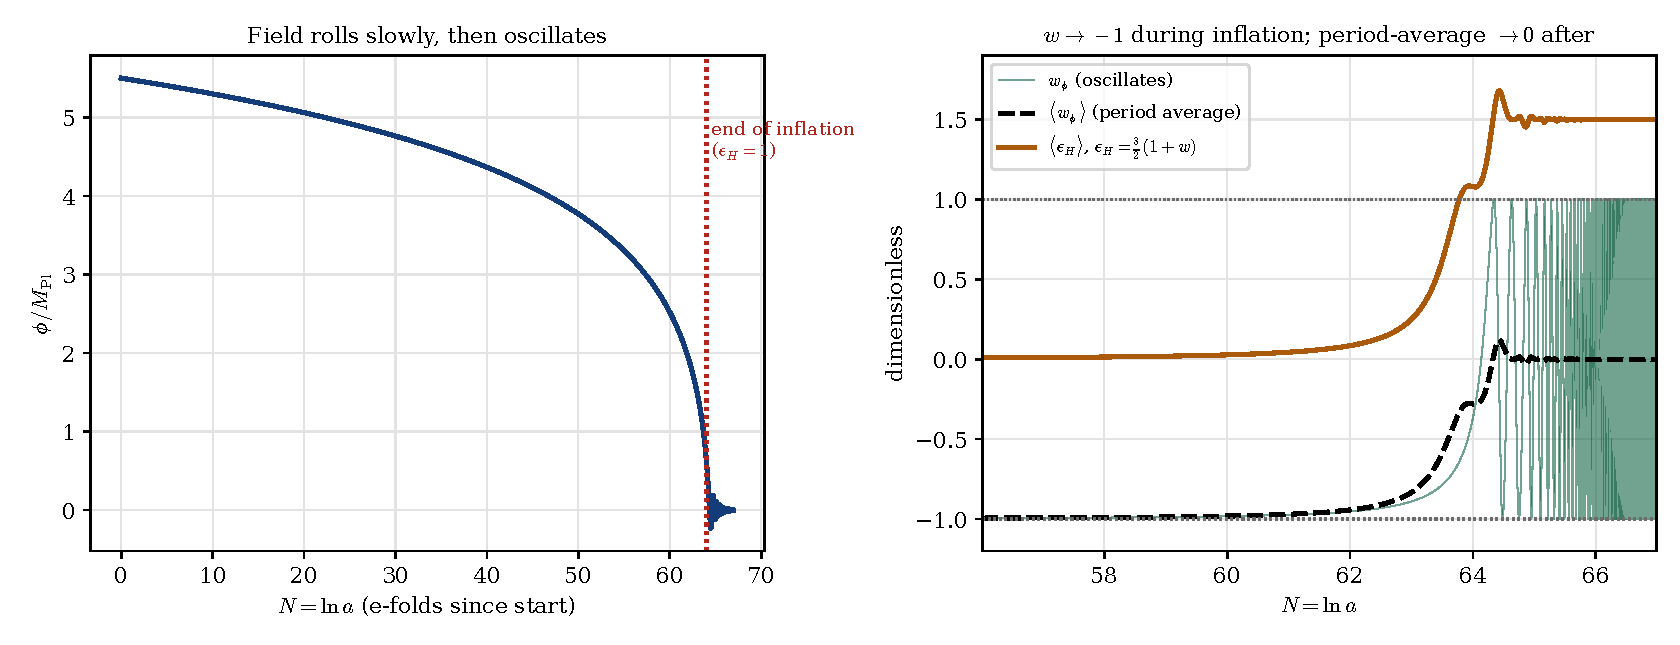
\includegraphics[width=0.9\textwidth]{figs/fig_infl_dyn.pdf}
\caption{\small דינמיקה של שדה האינפלטון: גלגול איטי, סוף האינפלציה ב-$\epsilon=1$, ותנודות.}
\end{figure}

\subsection{הפרעות}
האינפלציה לא רק מחליקה --- היא גם זורעת. תנודות קוונטיות של $\phi$ על רקע דה-סיטר:
\begin{equation}
\delta\phi\simeq\frac{H}{2\pi}\quad\text{לכל \en{e-fold}, ביציאה מהאופק }(k=aH).
\end{equation}
הן הופכות להפרעת עקמומיות $\mathcal R=-H\,\delta\phi/\dot\phi$, שנשמרת מעל האופק (הרצאה 3) עד שהמוד חוזר פנימה בעידן הקרינה וזורע את גלי הקול של הרצאה 5.
\begin{keybox}
\begin{align}
\Delta^2_{\mathcal R}(k)&=\frac{H^2}{8\pi^2\epsilon M_{\rm Pl}^2}\bigg|_{k=aH}=\frac{V}{24\pi^2\epsilon M_{\rm Pl}^4}\equiv A_s\Big(\frac{k}{k_*}\Big)^{n_s-1},
&
n_s-1&=2\eta_V-6\epsilon_V,\\
\Delta^2_t(k)&=\frac{2H^2}{\pi^2M_{\rm Pl}^2}\quad(\text{גלי כבידה}),
&
r&\equiv\frac{\Delta_t^2}{\Delta_{\mathcal R}^2}=16\epsilon_V,\quad n_t=-2\epsilon_V .
\end{align}
\end{keybox}
\textbf{היגיון ה-$n_s$:} $H$ ו-$\epsilon$ משתנים לאט במהלך האינפלציה, ולכן הספקטרום \emph{כמעט} אינווריאנטי לסולם, עם סטייה קטנה בשיעור $\epsilon,\eta\sim1/N$. ו-$r$ מודד ישירות את סולם האנרגיה: $V^{1/4}\approx1.0\times10^{16}\,\mathrm{GeV}\,(r/0.01)^{1/4}$.

\subsection{תחזיות ותצפיות}
\begin{center}\small
\begin{tabular}{@{}p{5.4cm}p{5cm}p{5.4cm}@{}}
\toprule
תחזית & מדוע & תצפית \\ \midrule
יקום שטוח & $|\Omega-1|\propto e^{-2N}$ & $\Omega_k=0.001\pm0.002$ \\
הפרעות אדיאבטיות וגאוסיות & שדה יחיד, תנודות קוונטיות ליניאריות & $f_{\rm NL}^{\rm loc}=-0.9\pm5.1$ \\
כמעט אינווריאנטי לסולם, "אדום" ($n_s<1$) & $H$ יורד לאט & $n_s=0.965\pm0.004$ (\en{Planck 2018}) \\
הפרעות מעבר לאופק ב-$z_\star$ & נוצרו באינפלציה & מתאם \en{TE} בסולמות $>1^\circ$ \\
גלי כבידה ($r$) & תנודות של המטריקה & $r<0.036$ (\en{BICEP/Keck 2021}) \\ \bottomrule
\end{tabular}
\end{center}
\textbf{מודלים.} $V=\tfrac12m^2\phi^2$: $n_s=1-2/N$, $r=8/N\approx0.13$ --- \textbf{נפסל}. \en{Starobinsky} ($R^2$): $n_s=1-2/N$, $r=12/N^2\approx0.003$ --- בלב האזור המותר. ניסויי \en{B-modes} הבאים (\en{Simons Observatory}, \en{LiteBIRD}) יגיעו ל-$r\sim10^{-3}$ ויבחנו את \en{Starobinsky} ישירות.

\begin{figure}[htbp]\centering
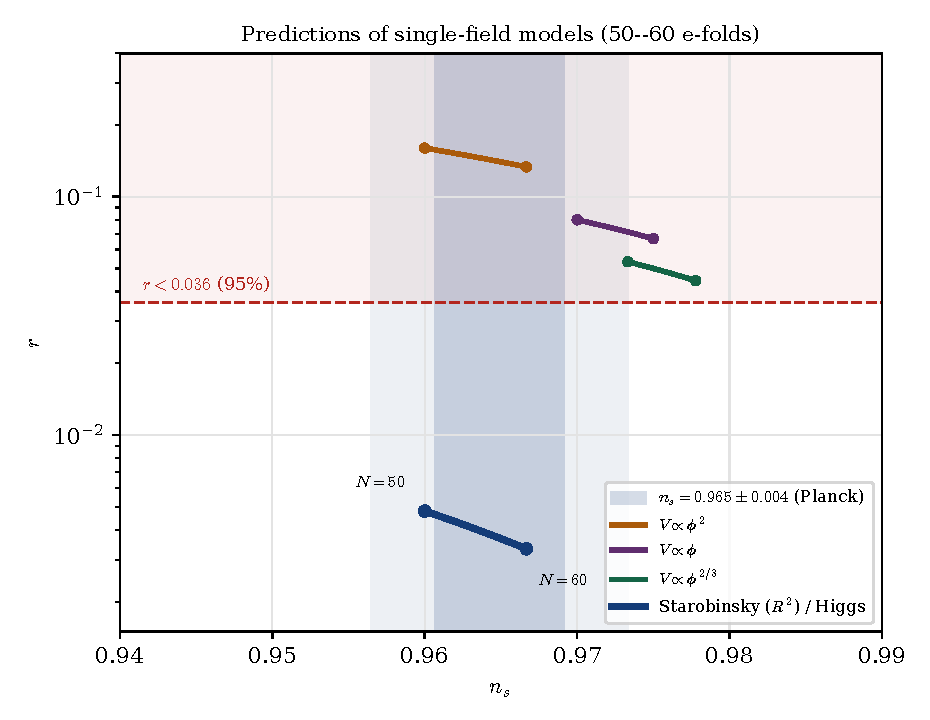
\includegraphics[width=0.6\textwidth]{figs/fig_infl_nsr.pdf}
\caption{\small המישור $(n_s,r)$: מודלים מול האזור המותר.}
\end{figure}

\begin{warnbox}
\textbf{מה אינפלציה לא פותרת.} את הקבוע הקוסמולוגי היום; את שאלת תנאי ההתחלה לאינפלציה עצמה; ואת זהות האינפלטון. היא מסגרת, לא מודל אחד.
\end{warnbox}

% ---------------------------------------------------------------------
\subsection*{תרגילים}
\begin{exercise}{כמה כוונון עדין?}
היום $|\Omega_k|<0.002$. (א) השתמשו ב-$|\Omega-1|\propto a$ (חומר) ו-$\propto a^2\propto T^{-2}$ (קרינה) כדי להעריך את $|\Omega-1|$ ב-\en{BBN} ($T=1\,\mathrm{MeV}$) ובזמן פלאנק ($T=10^{19}\,\mathrm{GeV}$); $T_{\rm eq}\approx0.8\,\mathrm{eV}$. (ב) כמה \en{e-folds} של אינפלציה מספיקים כדי ש-$|\Omega-1|=1$ לפניה ייתן את הערך מ-(א) אחריה, בסולם $T\sim10^{15}\,\mathrm{GeV}$?
\end{exercise}
\begin{solbox}
\textbf{פתרון.}\ (א) חומר: $|\Omega-1|_{\rm eq}=0.002/3400=6\times10^{-7}$. קרינה: $\times(T_{\rm eq}/T)^2$. \en{BBN}: $(0.8\,\mathrm{eV}/1\,\mathrm{MeV})^2=6.4\times10^{-13}\Rightarrow4\times10^{-19}$. פלאנק: עוד $(10^{-3}/10^{19})^2=10^{-44}\Rightarrow4\times10^{-63}$.\\
(ב) ב-$10^{15}\,\mathrm{GeV}$: $4\times10^{-19}\times(10^{-3}/10^{15})^2=4\times10^{-55}$. $e^{-2N}=4\times10^{-55}\Rightarrow N\approx63$. מכאן "60 \en{e-folds}".
\end{solbox}

\begin{exercise}{אינפלציה ריבועית, $V=\tfrac12m^2\phi^2$}
(א) חשבו $\epsilon_V$, $\eta_V$, ו-$\phi_{\rm end}$ (שבו $\epsilon_V=1$). (ב) הראו ש-$N(\phi)=(\phi^2-\phi_{\rm end}^2)/4M_{\rm Pl}^2$, ומצאו $\phi_*$ עבור $N=60$. האם השדה גדול ממסת פלאנק? (ג) חשבו $n_s$ ו-$r$. האם המודל מותר? (ד) מ-$A_s=2.1\times10^{-9}$ חשבו $m$.
\end{exercise}
\begin{solbox}
\textbf{פתרון.}\ (א) $\epsilon_V=\eta_V=2M_{\rm Pl}^2/\phi^2$; $\phi_{\rm end}=\sqrt2M_{\rm Pl}$.\\
(ב) $N=\int\frac{\phi}{2M_{\rm Pl}^2}d\phi=\frac{\phi_*^2-\phi_{\rm end}^2}{4M_{\rm Pl}^2}$; $\phi_*=\sqrt{4N+2}\,M_{\rm Pl}=15.6\,M_{\rm Pl}$: על-פלאנקי (אבל $V\ll M_{\rm Pl}^4$).\\
(ג) $n_s=1-8/(4N+2)\approx1-2/N=0.967$; $r=32/(4N+2)\approx8/N=0.13$. $n_s$ בסדר, אבל $r>0.036$: נפסל.\\
(ד) $\Delta^2_{\mathcal R}=\frac{V}{24\pi^2\epsilon_VM_{\rm Pl}^4}=\frac{m^2\phi_*^4}{96\pi^2M_{\rm Pl}^6}$ $\Rightarrow m=\sqrt{96\pi^2A_s}\,M_{\rm Pl}^3/\phi_*^2=5.8\times10^{-6}M_{\rm Pl}=1.4\times10^{13}\,\mathrm{GeV}$.
\end{solbox}

\begin{exercise}{\en{Starobinsky}}
$V=V_0\big(1-e^{-\sqrt{2/3}\,\phi/M_{\rm Pl}}\big)^2$. (א) בגבול $\phi\gg M_{\rm Pl}$, הראו $\epsilon_V\simeq\tfrac43e^{-2\sqrt{2/3}\phi/M_{\rm Pl}}$ ו-$\eta_V\simeq-\tfrac43e^{-\sqrt{2/3}\phi/M_{\rm Pl}}$. (ב) הראו $N\simeq\tfrac34e^{\sqrt{2/3}\phi/M_{\rm Pl}}$ ומכאן $n_s\simeq1-2/N$, $r\simeq12/N^2$. (ג) הציבו $N=55$ והשוו לטבלה.
\end{exercise}
\begin{solbox}
\textbf{פתרון.}\ (א) עם $\alpha=\sqrt{2/3}/M_{\rm Pl}$ ו-$e^{-\alpha\phi}\ll1$: $V'/V\simeq2\alpha e^{-\alpha\phi}$, $V''/V\simeq-2\alpha^2e^{-\alpha\phi}$. מכאן $\epsilon_V=2\alpha^2M_{\rm Pl}^2e^{-2\alpha\phi}=\tfrac43e^{-2\alpha\phi}$, $\eta_V=-\tfrac43e^{-\alpha\phi}$.\\
(ב) $N\simeq\int\frac{e^{\alpha\phi}}{2\alpha M_{\rm Pl}^2}d\phi=\tfrac34e^{\alpha\phi}$. אז $\eta_V=-1/N$, $\epsilon_V=3/4N^2$: $n_s=1+2\eta-6\epsilon\simeq1-2/N$, $r=16\epsilon=12/N^2$.\\
(ג) $N=55$: $n_s=0.964$, $r=0.004$ --- בתוך האזור המותר, ומטרה ל-\en{LiteBIRD}.
\end{solbox}


\clearpage
\section*{נספח: קבועים ונוסחאות}
\addcontentsline{toc}{section}{נספח: קבועים ונוסחאות}
\begin{center}\small
\begin{tabular}{@{}ll@{}}
\toprule
$G=6.674\times10^{-11}\,\mathrm{m^3\,kg^{-1}\,s^{-2}}=4.30\times10^{-6}\,\kpc\,(\kms)^2/\Msun$ & $1\,\Mpc=3.086\times10^{22}\,\mathrm m$ \\
$\rho_{c,0}=3H_0^2/8\pi G=1.878\times10^{-26}h^2\,\mathrm{kg\,m^{-3}}=2.775\times10^{11}h^2\,\Msun\,\Mpc^{-3}$ & $\Msun=1.989\times10^{30}\,\mathrm{kg}$ \\
$T_0=2.7255\,\mathrm K$, \ $\Omega_\gamma h^2=2.47\times10^{-5}$, \ $\Omega_rh^2\simeq4.2\times10^{-5}$ (עם נייטרינו) & $k_B=8.617\times10^{-5}\,\mathrm{eV\,K^{-1}}$ \\
$M_{\rm Pl}=(8\pi G)^{-1/2}=2.435\times10^{18}\,\mathrm{GeV}$ (מסת פלאנק המוקטנת) & $1\,\mathrm{yr}=3.156\times10^7\,\mathrm s$ \\
\bottomrule
\end{tabular}
\end{center}

\subsection*{לקריאה}
\begin{itemize}
\item \en{B. Ryden, \emph{Introduction to Cosmology}, 2nd ed.\ (Cambridge, 2017)} --- הרצאות 1, 4, 5.
\item \en{D. Baumann, \emph{Cosmology} (Cambridge, 2022)} --- הרצאות 3, 5, 6.
\item \en{D.~W. Hogg, \emph{Distance measures in cosmology}, arXiv:astro-ph/9905116} --- הרצאה 1.
\item \en{Foreman-Mackey et al.\ 2013, PASP 125, 306 (\texttt{emcee}); Brout et al.\ 2022, ApJ 938, 110 (Pantheon+)} --- הרצאה 2.
\item \en{Kahn \& Woltjer 1959, ApJ 130, 705; Gunn \& Gott 1972, ApJ 176, 1; Lahav et al.\ 1991, MNRAS 251, 128; Bryan \& Norman 1998, ApJ 495, 80; Li \& White 2008, MNRAS 384, 1459; Pavlidou \& Tomaras 2014, JCAP 09, 020; Naderi, Malekjani \& Pace 2015, MNRAS 447, 1873} --- הרצאה 4 (קריסה כדורית).
\item \en{Navarro, Frenk \& White 1997, ApJ 490, 493; Famaey \& McGaugh 2012, Living Rev.\ Rel.\ 15, 10} --- הרצאה 4.
\item \en{DESI Collaboration 2025, arXiv:2503.14738 (DR2 BAO)} --- הרצאה 5.
\end{itemize}

\end{document}
